\section{Porównanie wykorzystanych algorytmów}

Badania zostały przeprowadzone na komputerze Politechniki Poznańskiej przygotowanym do 
wykonywania dużych obliczeń (HPC --- High Performance Compuning). Dane pochodzą z plików
TSP ze strony http://comopt.ifi.uni-heidelberg.de/software/TSPLIB95/, ponieważ znane są dla
nich rozwiązania optymalne. Dane te były wczytywane przez program i na nich wykonywane były 
obliczenia. Algorytmy Greedy i Steepest uruchamiane były 10 razy, za każdym razem i innym 
punktem początkowym. Algorytm Random uruchamiany był 10 razy, za każdym razem z innym 
limitem powtórzeń (od 20~000 do 200~000). Ostatnim algorytmem była prosta Heurystyka, również uruchamiana 10 razy, za każdym razem z innym miastem początkowym.

\subsection{Odległość od optimum}

Odległość od optimum mierzone było na plikach TSP ze znanymi rozwiązaniami. Każdy algorytm 
uruchamiany był 10 razy, aby uniknąć przekłamania wynikającego z jednorazowego znalezienia 
optimum lokalnego. przedstawione wyniki są najlepszymi, uśrednionymi i najgorszymi.

Procentową odległość od optimum wyliczono dzięki następującemu wzorowi:

$$ \frac{f_{obliczone} - f_{optymalne}}{f_{optymalne}} * 100 \% $$


Uzyskane wyniki przedstawiono na rysunkach \ref{greedy_sort_best}, \ref{own_results}, \ref{steepest_sort_best}, 
\ref{random_sort_best}, \ref{greedy_av_sort},  \ref{steepest_av_sort}, 
\ref{random_av_sort}, \ref{greedy_sort_worst},
\ref{steepest_sort_worst}, \ref{random_sort_worst}, \ref{best_com} i \ref{av_comp}. % i \ref{worst_comp}.

\begin{adjustwidth}{-1in}{-1in}%

\begin{center}

\begin{tabular}{lcccccccccc}

\toprule
 \multirow{2}{*}{Dane TSP} & \multirow{2}{*}{Rozmiar} & \multirow{2}{*}{Optimum} & \multicolumn{2}{c}{Greedy} & \multicolumn{2}{c}{Steepest} & \multicolumn{2}{c}{Autorski} & \multicolumn{2}{c}{Losowy} \\
 & & & Wynik & \% & Wynik & \% & Wynik & \% & Wynik & \% \\
\toprule
\multirow{3}{*}{eil51} & \multirow{3}{*}{51} & \multirow{3}{*}{426} & 572 & 34,3  & 505 & 18,5  & 548 & 28,6  & 1226 & 187,8 \\
 & &  & 572 & 34,3  & 526,6 & 23,6  & 548 & 28,6  & 1249,8 & 193,4 \\
 & &  & 572 & 34,3  & 541 & 27  & 548 & 28,6  & 1299 & 204,9 \\
\midrule
\multirow{3}{*}{berlin52} & \multirow{3}{*}{52} & \multirow{3}{*}{7542} & 10373 & 37,5  & 10132 & 34,3  & 8164 & 8,2  & 21933 & 190,8 \\
 & &  & 11244,2 & 49,1  & 10441,2 & 38,4  & 8164 & 8,2  & 22574,6 & 199,3 \\
 & &  & 11462 & 52  & 10905 & 44,6  & 8164 & 8,2  & 22940 & 204,2 \\
\midrule
\multirow{3}{*}{eil76} & \multirow{3}{*}{76} & \multirow{3}{*}{538} & 692 & 28,6  & 737 & 37  & 684 & 27,1  & 1860 & 245,7 \\
 & &  & 731,1 & 35,9  & 800,1 & 48,7  & 684 & 27,1  & 1967,6 & 265,7 \\
 & &  & 777 & 44,4  & 885 & 64,5  & 684 & 27,1  & 2004 & 272,5 \\
\midrule
\multirow{3}{*}{pr76} & \multirow{3}{*}{76} & \multirow{3}{*}{108159} & 163066 & 50,8  & 153827 & 42,2  & 150825 & 39,4  & 444502 & 311 \\
 & &  & 166916,6 & 54,3  & 168609 & 55,9  & 150825 & 39,4  & 454662 & 320,4 \\
 & &  & 176535 & 63,2  & 175278 & 62,1  & 150825 & 39,4  & 475826 & 339,9 \\
\midrule
\multirow{3}{*}{rat99} & \multirow{3}{*}{99} & \multirow{3}{*}{1211} & 1855 & 53,2  & 2005 & 65,6  & 1596 & 31,8  & 6402 & 428,7 \\
 & &  & 1972,4 & 62,9  & 2151,7 & 77,7  & 1596 & 31,8  & 6561,3 & 441,8 \\
 & &  & 2135 & 76,3  & 2454 & 102,6  & 1596 & 31,8  & 6762 & 458,4 \\
\midrule
\multirow{3}{*}{kroA100} & \multirow{3}{*}{100} & \multirow{3}{*}{21282} & 30010 & 41  & 40736 & 91,4  & 28656 & 34,6  & 131710 & 518,9 \\
 & &  & 36768,1 & 72,8  & 45334,8 & 113  & 28656 & 34,6  & 134689,9 & 532,9 \\
 & &  & 40163 & 88,7  & 51553 & 142,2  & 28656 & 34,6  & 136550 & 541,6 \\
\midrule
\multirow{3}{*}{kroB100} & \multirow{3}{*}{100} & \multirow{3}{*}{22141} & 32956 & 48,8  & 39026 & 76,3  & 26832 & 21,2  & 130394 & 488,9 \\
 & &  & 40005,8 & 80,7  & 44381,9 & 100,5  & 26832 & 21,2  & 134289,1 & 506,5 \\
 & &  & 45617 & 106  & 48969 & 121,2  & 26832 & 21,2  & 136182 & 515,1 \\
\midrule
\multirow{3}{*}{kroC100} & \multirow{3}{*}{100} & \multirow{3}{*}{20749} & 37723 & 81,8  & 37876 & 82,5  & 26086 & 25,7  & 129739 & 525,3 \\
 & &  & 41489,4 & 100  & 43303,5 & 108,7  & 26086 & 25,7  & 133786,9 & 544,8 \\
 & &  & 45072 & 117,2  & 53572 & 158,2  & 26086 & 25,7  & 136309 & 556,9 \\
\bottomrule

\end{tabular}


\begin{tabular}{lcccccccccc}

\toprule
 \multirow{2}{*}{Dane TSP} & \multirow{2}{*}{Rozmiar} & \multirow{2}{*}{Optimum} & \multicolumn{2}{c}{Greedy} & \multicolumn{2}{c}{Steepest} & \multicolumn{2}{c}{Autorski} & \multicolumn{2}{c}{Losowy} \\
 & & & Wynik & \% & Wynik & \% & Wynik & \% & Wynik & \% \\
\toprule
\multirow{3}{*}{kroD100} & \multirow{3}{*}{100} & \multirow{3}{*}{21294} & 33284 & 56,3  & 33788 & 58,7  & 25671 & 20,6  & 127314 & 497,9 \\
 & &  & 39281,2 & 84,5  & 41584 & 95,3  & 25671 & 20,6  & 128608,3 & 504 \\
 & &  & 46571 & 118,7  & 46696 & 119,3  & 25671 & 20,6  & 130886 & 514,7 \\
\midrule
\multirow{3}{*}{kroE100} & \multirow{3}{*}{100} & \multirow{3}{*}{22068} & 34078 & 54,4  & 36313 & 64,6  & 28859 & 30,8  & 130490 & 491,3 \\
 & &  & 37439,8 & 69,7  & 40933,7 & 85,5  & 28859 & 30,8  & 134750,7 & 510,6 \\
 & &  & 42585 & 93  & 45025 & 104  & 28859 & 30,8  & 139542 & 532,3 \\
\midrule
\multirow{3}{*}{eil101} & \multirow{3}{*}{101} & \multirow{3}{*}{629} & 830 & 32  & 871 & 38,5  & 781 & 24,2  & 2677 & 325,6 \\
 & &  & 890,3 & 41,5  & 939,5 & 49,4  & 781 & 24,2  & 2778,1 & 341,7 \\
 & &  & 966 & 53,6  & 1012 & 60,9  & 781 & 24,2  & 2817 & 347,9 \\
\midrule
\multirow{3}{*}{lin105} & \multirow{3}{*}{105} & \multirow{3}{*}{14379} & 23455 & 63,1  & 24839 & 72,7  & 18657 & 29,8  & 96137 & 568,6 \\
 & &  & 26634,1 & 85,2  & 29502 & 105,2  & 18657 & 29,8  & 98617,9 & 585,8 \\
 & &  & 31651 & 120,1  & 33872 & 135,6  & 18657 & 29,8  & 100969 & 602,2 \\
\midrule
\multirow{3}{*}{pr107} & \multirow{3}{*}{107} & \multirow{3}{*}{44303} & 121704 & 174,7  & 126661 & 185,9  & 49734 & 12,3  & 414762 & 836,2 \\
 & &  & 142059,7 & 220,7  & 164989,3 & 272,4  & 49734 & 12,3  & 443736,3 & 901,6 \\
 & &  & 167142 & 277,3  & 191224 & 331,6  & 49734 & 12,3  & 460395 & 939,2 \\
\midrule
\multirow{3}{*}{pr124} & \multirow{3}{*}{124} & \multirow{3}{*}{59030} & 115163 & 95,1  & 151116 & 156  & 70689 & 19,8  & 554291 & 839 \\
 & &  & 138572,8 & 134,7  & 168236,7 & 185  & 70689 & 19,8  & 570714,6 & 866,8 \\
 & &  & 154631 & 162  & 185514 & 214,3  & 70689 & 19,8  & 592184 & 903,2 \\
\midrule
\multirow{3}{*}{bier127} & \multirow{3}{*}{127} & \multirow{3}{*}{118282} & 164520 & 39,1  & 166630 & 40,9  & 147570 & 24,8  & 531521 & 349,4 \\
 & &  & 174341,5 & 47,4  & 184839,6 & 56,3  & 147570 & 24,8  & 538922,2 & 355,6 \\
 & &  & 182785 & 54,5  & 215233 & 82  & 147570 & 24,8  & 547164 & 362,6 \\
\midrule
\multirow{3}{*}{pr136} & \multirow{3}{*}{136} & \multirow{3}{*}{96772} & 158288 & 63,6  & 161110 & 66,5  & 123399 & 27,5  & 670718 & 593,1 \\
 & &  & 176393,1 & 82,3  & 200869,6 & 107,6  & 123399 & 27,5  & 687914,9 & 610,9 \\
 & &  & 190062 & 96,4  & 229552 & 137,2  & 123399 & 27,5  & 701454 & 624,9 \\
\midrule
\multirow{3}{*}{pr144} & \multirow{3}{*}{144} & \multirow{3}{*}{58537} & 150361 & 156,9  & 182928 & 212,5  & 61665 & 5,3  & 672274 & 1048,5 \\
 & &  & 171255,8 & 192,6  & 201707,2 & 244,6  & 61665 & 5,3  & 677555,1 & 1057,5 \\
 & &  & 189675 & 224  & 227929 & 289,4  & 61665 & 5,3  & 685471 & 1071 \\
\midrule
\multirow{3}{*}{kroA150} & \multirow{3}{*}{150} & \multirow{3}{*}{26524} & 46062 & 73,7  & 51998 & 96  & 33761 & 27,3  & 210578 & 693,9 \\
 & &  & 53938,1 & 103,4  & 59675,7 & 125  & 33761 & 27,3  & 213830,7 & 706,2 \\
 & &  & 63384 & 139  & 68980 & 160,1  & 33761 & 27,3  & 215742 & 713,4 \\
\midrule
\multirow{3}{*}{kroB150} & \multirow{3}{*}{150} & \multirow{3}{*}{26130} & 43418 & 66,2  & 50374 & 92,8  & 35925 & 37,5  & 206901 & 691,8 \\
 & &  & 49767,7 & 90,5  & 58716,8 & 124,7  & 35925 & 37,5  & 210747,4 & 706,5 \\
 & &  & 56998 & 118,1  & 68254 & 161,2  & 35925 & 37,5  & 216298 & 727,8 \\
\midrule
\multirow{3}{*}{pr152} & \multirow{3}{*}{152} & \multirow{3}{*}{73682} & 194334 & 163,7  & 228449 & 210  & 86740 & 17,7  & 874527 & 1086,9 \\
 & &  & 230673,8 & 213,1  & 263257,9 & 257,3  & 86740 & 17,7  & 885380,1 & 1101,6 \\
 & &  & 282255 & 283,1  & 278018 & 277,3  & 86740 & 17,7  & 900243 & 1121,8 \\
\midrule
\multirow{3}{*}{kroA200} & \multirow{3}{*}{200} & \multirow{3}{*}{29368} & 56014 & 90,7  & 62116 & 111,5  & 38910 & 32,5  & 286507 & 875,6 \\
 & &  & 60639 & 106,5  & 73140,2 & 149  & 38910 & 32,5  & 289380,9 & 885,4 \\
 & &  & 64466 & 119,5  & 84057 & 186,2  & 38910 & 32,5  & 295576 & 906,5 \\
\midrule
\multirow{3}{*}{kroB200} & \multirow{3}{*}{200} & \multirow{3}{*}{29437} & 49077 & 66,7  & 63946 & 117,2  & 36548 & 24,2  & 278639 & 846,6 \\
 & &  & 60858,4 & 106,7  & 72089,6 & 144,9  & 36548 & 24,2  & 282642,1 & 860,2 \\
 & &  & 67982 & 130,9  & 79453 & 169,9  & 36548 & 24,2  & 287685 & 877,3 \\
\bottomrule

\end{tabular}


\begin{tabular}{lcccccccccc}

\toprule
 \multirow{2}{*}{Dane TSP} & \multirow{2}{*}{Rozmiar} & \multirow{2}{*}{Optimum} & \multicolumn{2}{c}{Greedy} & \multicolumn{2}{c}{Steepest} & \multicolumn{2}{c}{Autorski} & \multicolumn{2}{c}{Losowy} \\
 & & & Wynik & \% & Wynik & \% & Wynik & \% & Wynik & \% \\
\toprule
\multirow{3}{*}{pr226} & \multirow{3}{*}{226} & \multirow{3}{*}{80369} & 251309 & 212,7  & 332530 & 313,8  & 99260 & 23,5  & 1440155 & 1691,9 \\
 & &  & 304511,3 & 278,9  & 391912,2 & 387,6  & 99260 & 23,5  & 1461011,9 & 1717,9 \\
 & &  & 355085 & 341,8  & 450920 & 461,1  & 99260 & 23,5  & 1474233 & 1734,3 \\
\midrule
\multirow{3}{*}{gil262} & \multirow{3}{*}{262} & \multirow{3}{*}{2378} & 4626 & 94,5  & 5378 & 126,2  & 2916 & 22,6  & 23331 & 881,1 \\
 & &  & 4911,9 & 106,6  & 5901,5 & 148,2  & 2916 & 22,6  & 23649,8 & 894,5 \\
 & &  & 5370 & 125,8  & 6430 & 170,4  & 2916 & 22,6  & 24079 & 912,6 \\
\midrule
\multirow{3}{*}{pr264} & \multirow{3}{*}{264} & \multirow{3}{*}{49135} & 148553 & 202,3  & 226991 & 362  & 57869 & 17,8  & 917026 & 1766,3 \\
 & &  & 197204,2 & 301,4  & 244873,3 & 398,4  & 57869 & 17,8  & 943002,8 & 1819,2 \\
 & &  & 235390 & 379,1  & 280707 & 471,3  & 57869 & 17,8  & 956577 & 1846,8 \\
\midrule
\multirow{3}{*}{a280} & \multirow{3}{*}{280} & \multirow{3}{*}{2579} & 5346 & 107,3  & 6466 & 150,7  & 3194 & 23,8  & 29312 & 1036,6 \\
 & &  & 5886,4 & 128,2  & 7012 & 171,9  & 3194 & 23,8  & 29812,6 & 1056 \\
 & &  & 6266 & 143  & 7835 & 203,8  & 3194 & 23,8  & 30069 & 1065,9 \\
\midrule
\multirow{3}{*}{pr299} & \multirow{3}{*}{299} & \multirow{3}{*}{48191} & 105064 & 118  & 125650 & 160,7  & 60651 & 25,9  & 654734 & 1258,6 \\
 & &  & 115471,1 & 139,6  & 144038,4 & 198,9  & 60651 & 25,9  & 663078,9 & 1275,9 \\
 & &  & 127366 & 164,3  & 165008 & 242,4  & 60651 & 25,9  & 670753 & 1291,9 \\
\midrule
\multirow{3}{*}{lin318} & \multirow{3}{*}{318} & \multirow{3}{*}{42029} & 83088 & 97,7  & 103585 & 146,5  & 53312 & 26,8  & 522745 & 1143,8 \\
 & &  & 99323,1 & 136,3  & 123899,7 & 194,8  & 53312 & 26,8  & 526311,9 & 1152,3 \\
 & &  & 107831 & 156,6  & 139741 & 232,5  & 53312 & 26,8  & 533705 & 1169,8 \\
\midrule
\multirow{3}{*}{linhp318} & \multirow{3}{*}{318} & \multirow{3}{*}{41345} & 97350 & 135,5  & 109349 & 164,5  & 51684 & 25  & 519971 & 1157,6 \\
 & &  & 104842,3 & 153,6  & 124553 & 201,3  & 51684 & 25  & 525158,1 & 1170,2 \\
 & &  & 117535 & 184,3  & 132277 & 219,9  & 51684 & 25  & 532496 & 1187,9 \\
\midrule
\multirow{3}{*}{pr439} & \multirow{3}{*}{439} & \multirow{3}{*}{107217} & 265531 & 147,7  & 346169 & 222,9  & 146215 & 36,4  & 1707733 & 1492,8 \\
 & &  & 296942,9 & 177  & 381129,5 & 255,5  & 146215 & 36,4  & 1721305,3 & 1505,4 \\
 & &  & 328823 & 206,7  & 406657 & 279,3  & 146215 & 36,4  & 1735160 & 1518,4 \\
\midrule
\multirow{3}{*}{rat575} & \multirow{3}{*}{575} & \multirow{3}{*}{6773} & 13350 & 97,1  & 18325 & 170,6  & 8191 & 20,9  & 101840 & 1403,6 \\
 & &  & 15378,8 & 127,1  & 19063,2 & 181,5  & 8405,8 & 24,1  & 103398,9 & 1426,6 \\
 & &  & 17712 & 161,5  & 20015 & 195,5  & 8549 & 26,2  & 104191 & 1438,3 \\
\midrule
\multirow{3}{*}{rat783} & \multirow{3}{*}{783} & \multirow{3}{*}{8806} & 21585 & 145,1  & 26174 & 197,2  & 10737 & 21,9  & 161657 & 1735,8 \\
 & &  & 22892,5 & 160  & 31087,3 & 253  & 10737 & 21,9  & 165030,2 & 1774,1 \\
 & &  & 23897 & 171,4  & 34084 & 287,1  & 10737 & 21,9  & 167367 & 1800,6 \\
\toprule%
\multicolumn{3}{c}{\multirow{2}{*}{Średnie wyniki [\%]}} & \multicolumn{2}{c}{91,6} & \multicolumn{2}{c}{124,6} & \multicolumn{2}{c}{24,9} & \multicolumn{2}{c}{819,1} \\
\multicolumn{3}{c}{} & \multicolumn{2}{c}{118,0} & \multicolumn{2}{c}{155,0} & \multicolumn{2}{c}{25,0} & \multicolumn{2}{c}{837,2} \\
\multicolumn{3}{c}{} & \multicolumn{2}{c}{144,0} & \multicolumn{2}{c}{184,8} & \multicolumn{2}{c}{25,0} & \multicolumn{2}{c}{853,3} \\
\bottomrule



\end{tabular}

\end{center}

\end{adjustwidth}

\begin{figure}
\begin{center}
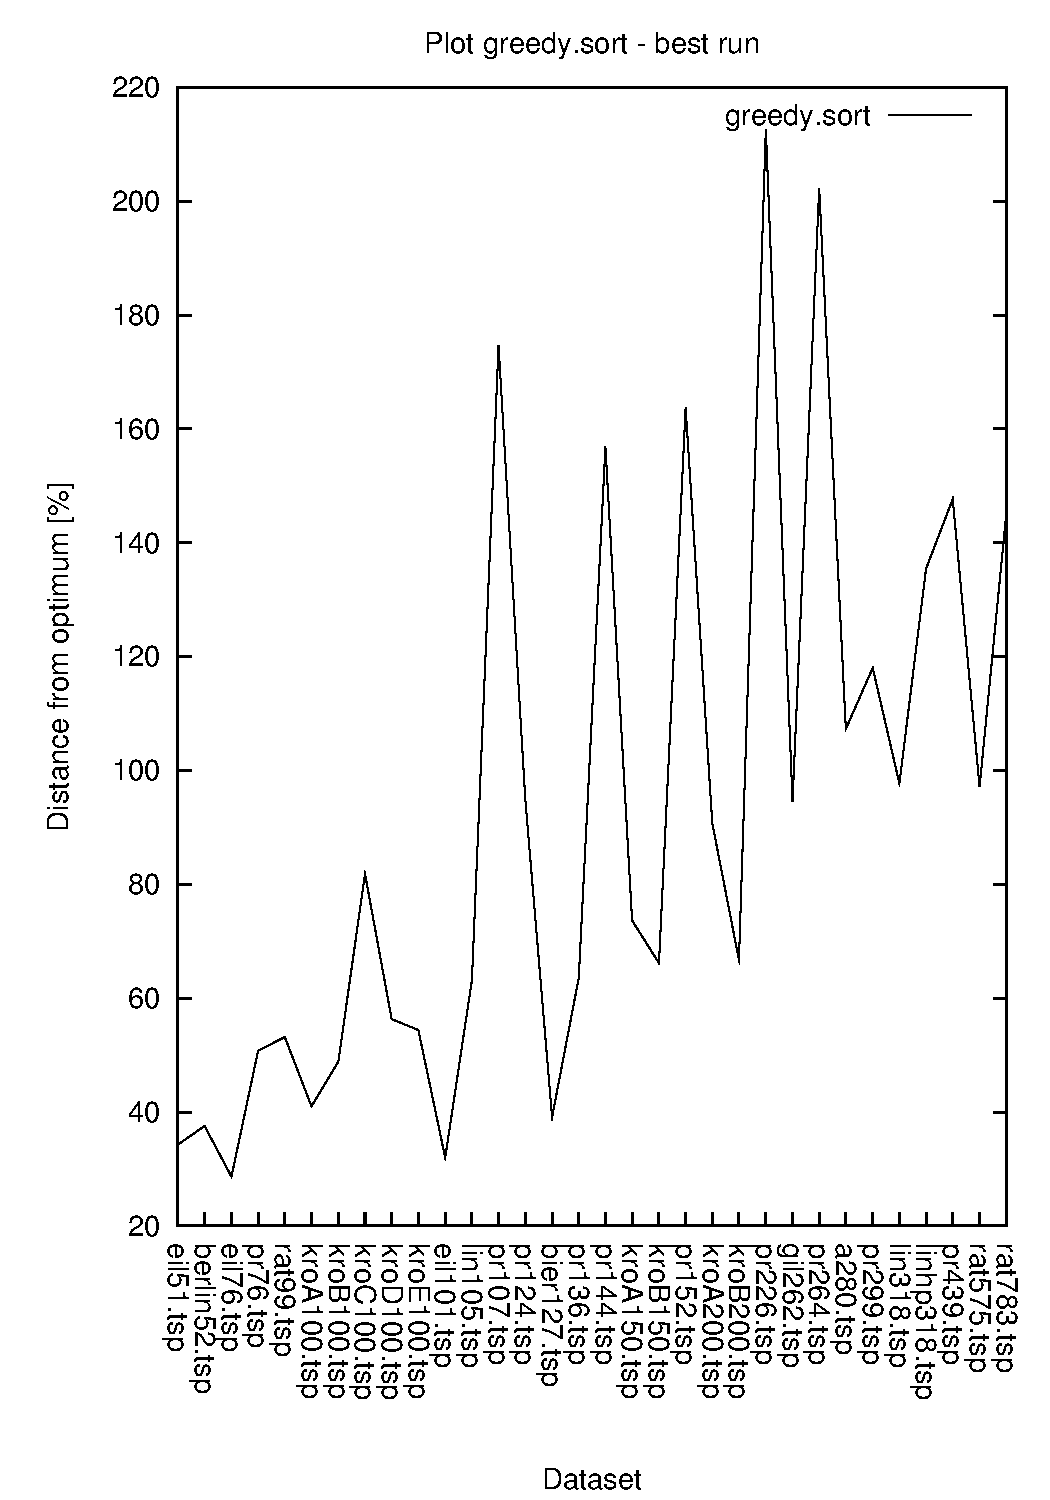
\includegraphics[width=0.9\textwidth]{wykresy/greedy_sort_best}
\end{center}
\caption{Najlepsza odległość od optimum dla algorytmu Greedy.}
\label{greedy_sort_best}
\end{figure}


\begin{figure}
\begin{center}
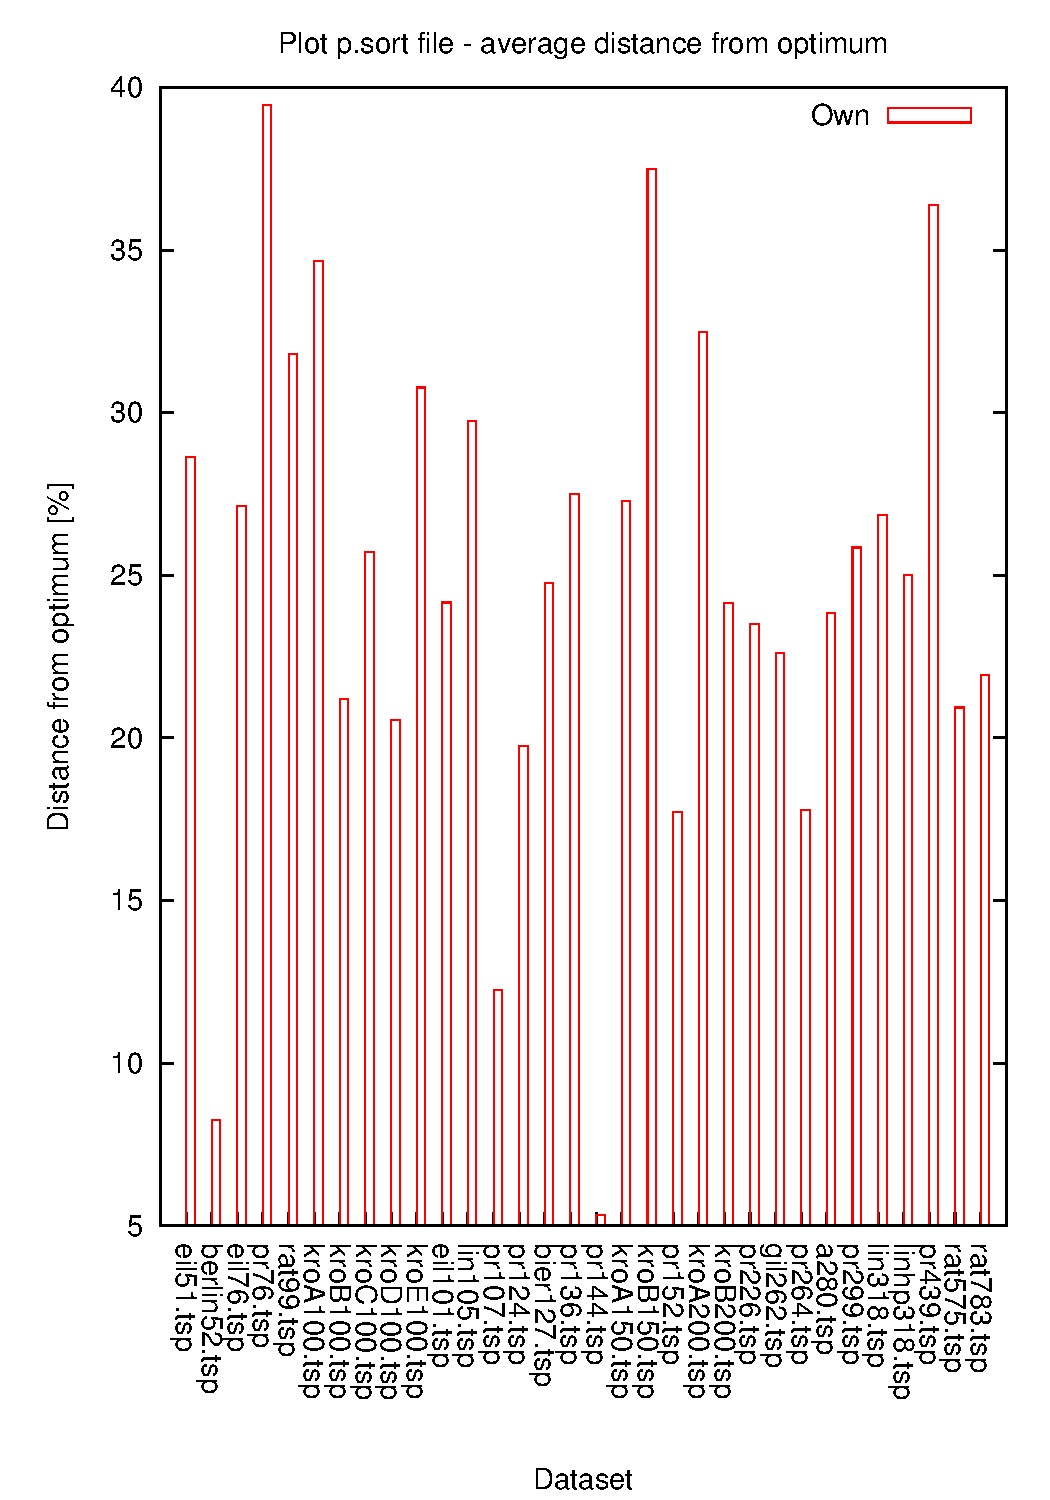
\includegraphics[width=0.9\textwidth]{wykresy/own_results}
\end{center}
\caption{Wyniki odległości od optimum dla prostej heurystyki.}
\label{own_results}
\end{figure}



\begin{figure}
\begin{center}
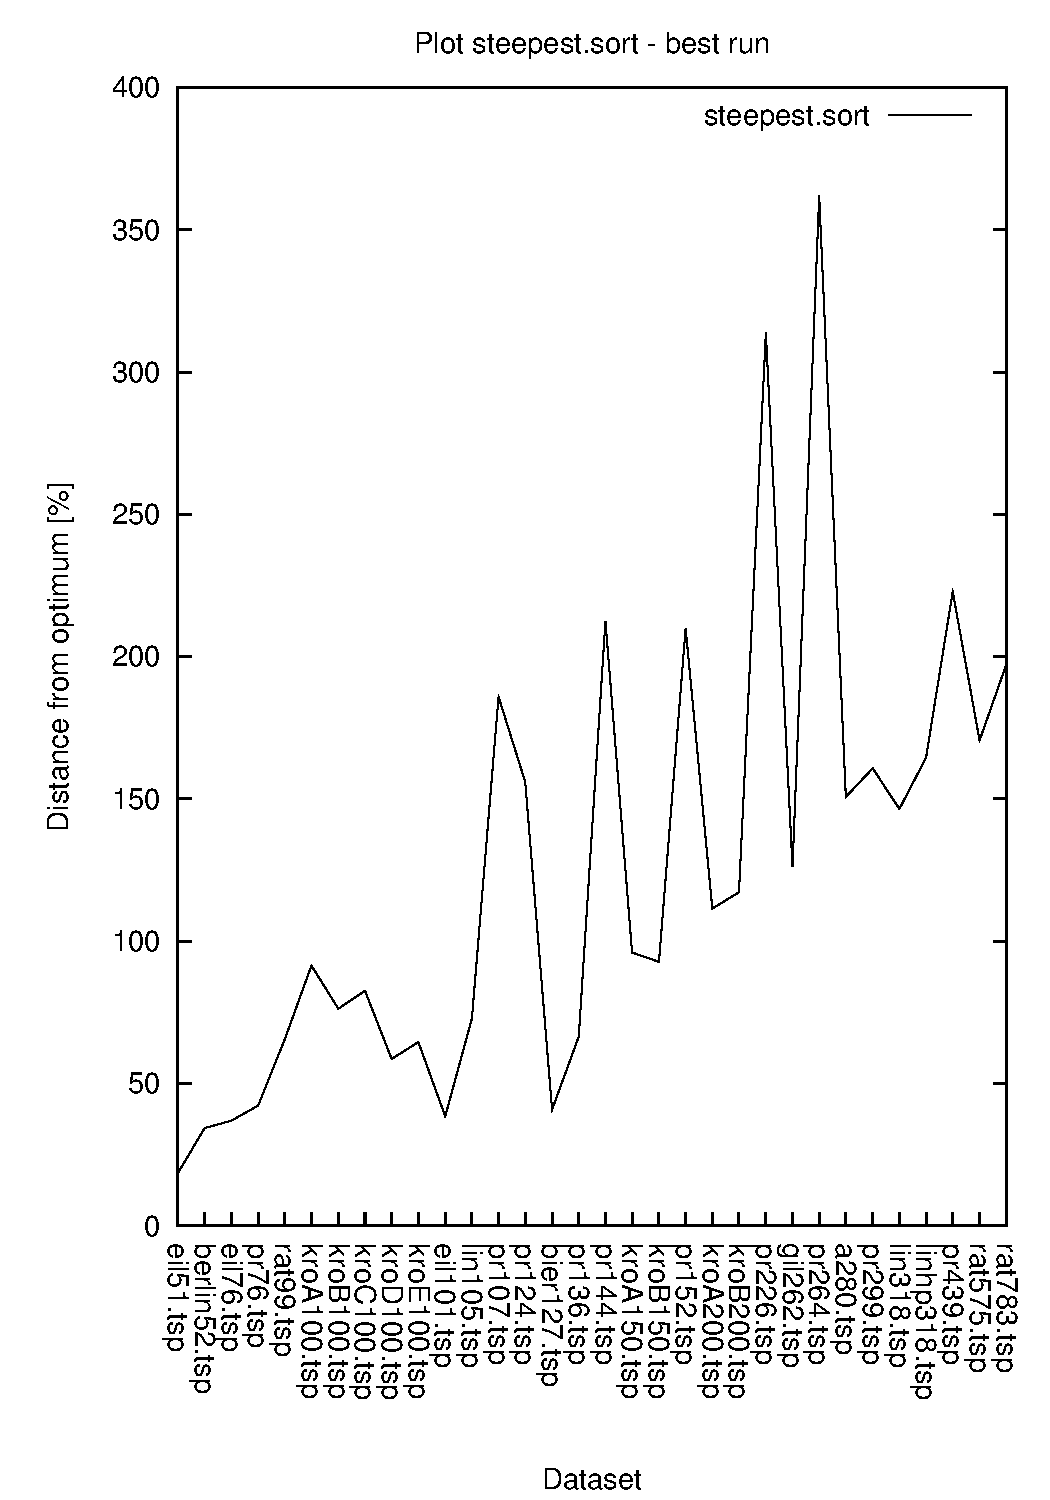
\includegraphics[width=0.9\textwidth]{wykresy/steepest_sort_best}
\end{center}
\caption{Najlepsza odległość od optimum dla algorytmu Steepest.}
\label{steepest_sort_best}
\end{figure}


\begin{figure}
\begin{center}
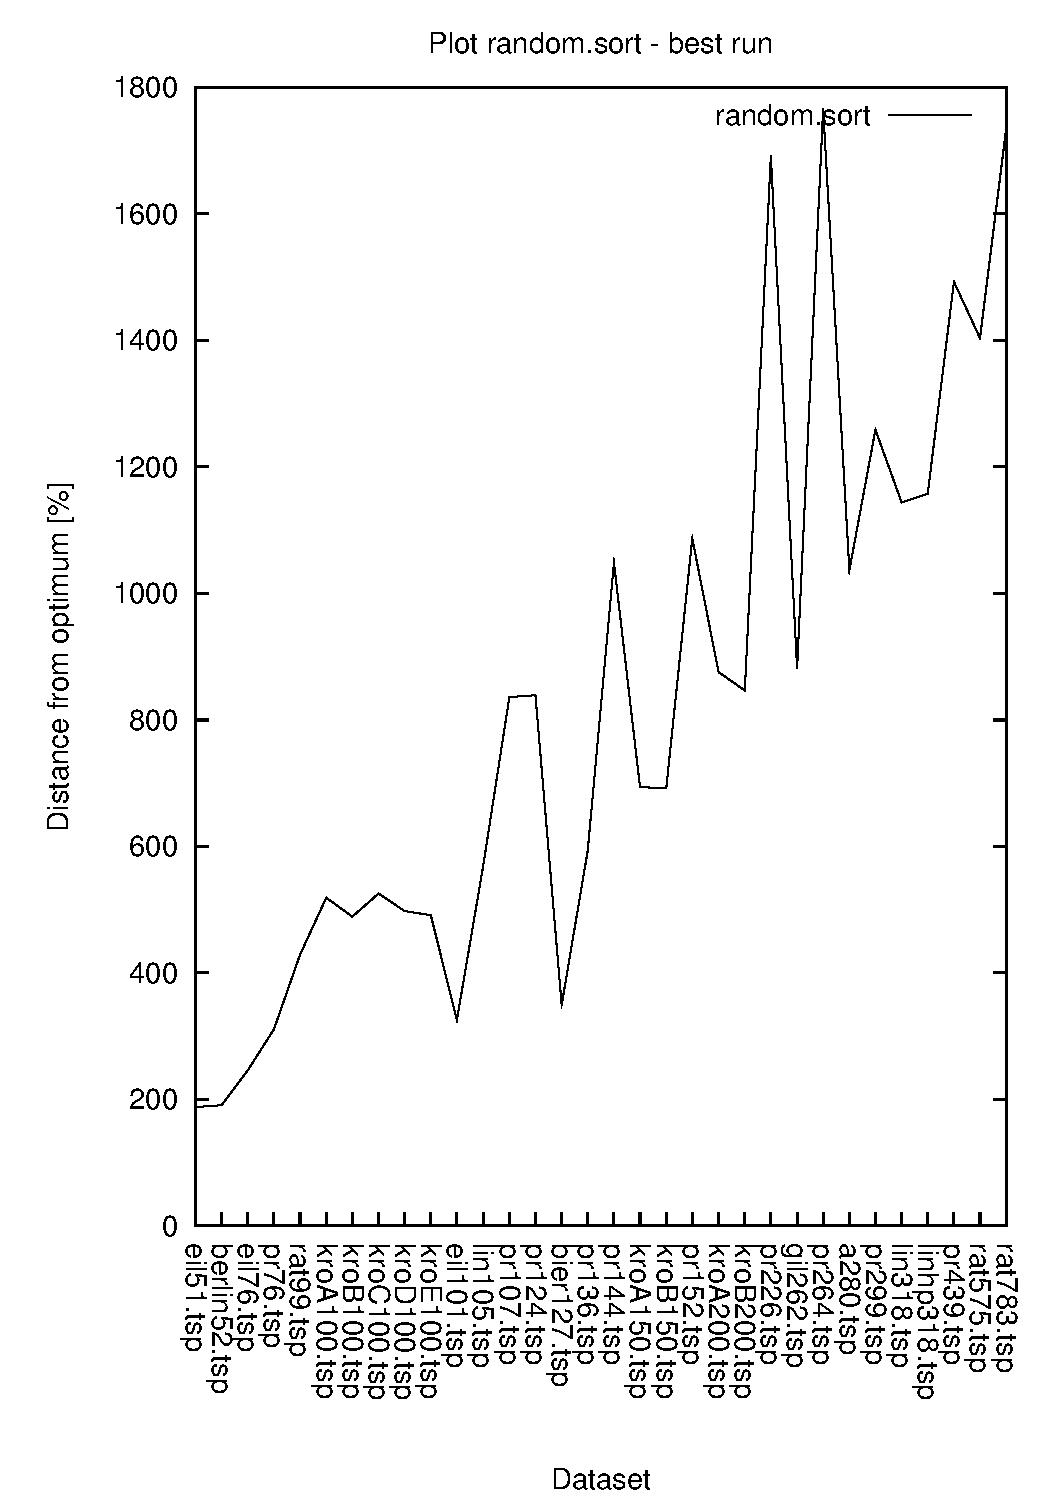
\includegraphics[width=0.9\textwidth]{wykresy/random_sort_best}
\end{center}
\caption{Najlepsza odległość od optimum dla algorytmu Random.}
\label{random_sort_best}
\end{figure}


\begin{figure}
\begin{center}
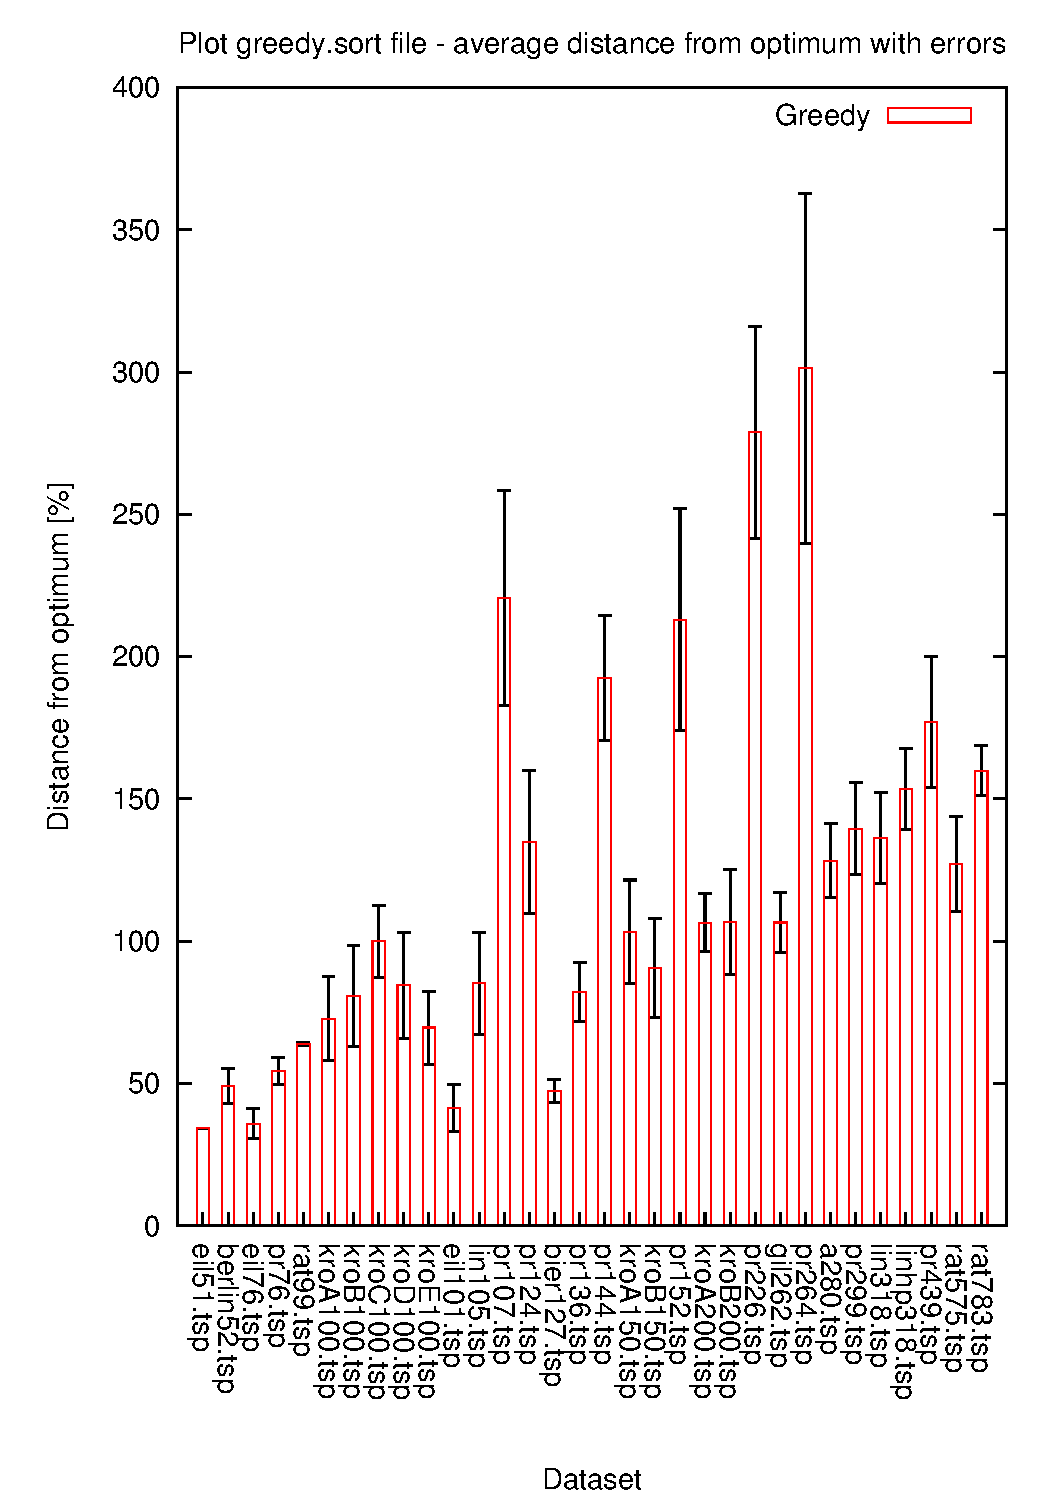
\includegraphics[width=0.9\textwidth]{wykresy/greedy_av_sort}
\end{center}
\caption{Średnia odległość od optimum dla algorytmu Greedy.}
\label{greedy_av_sort}
\end{figure}


\begin{figure}
\begin{center}
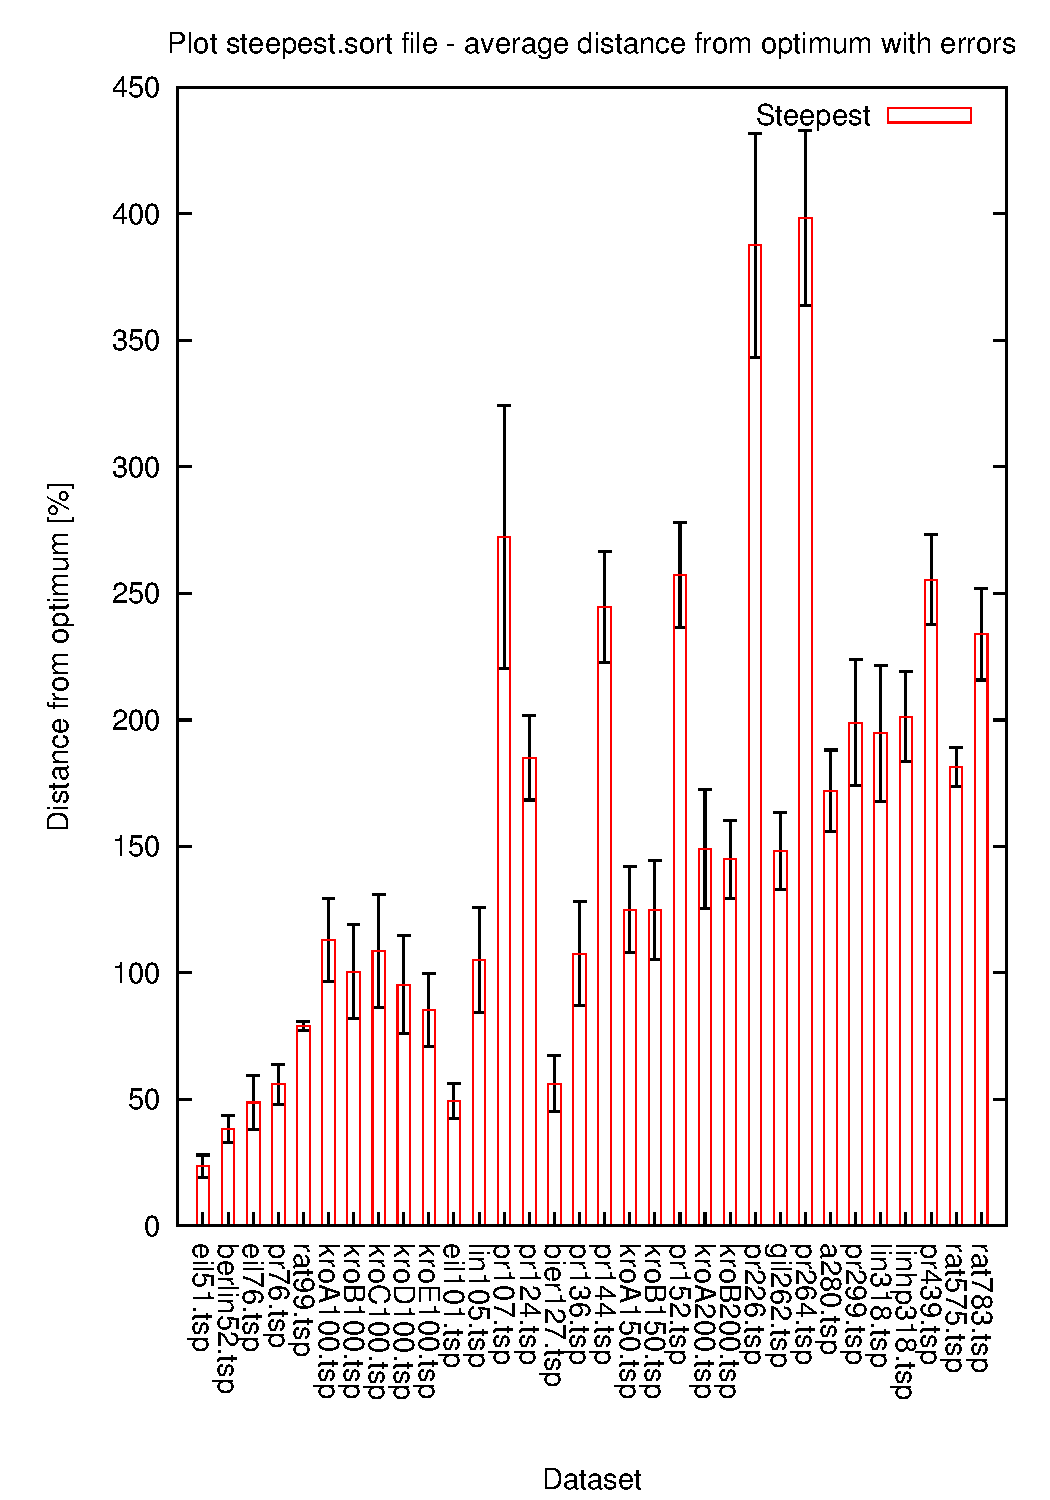
\includegraphics[width=0.9\textwidth]{wykresy/steepest_av_sort}
\end{center}
\caption{Średnia odległość od optimum dla algorytmu Steepest.}
\label{steepest_av_sort}
\end{figure}


\begin{figure}
\begin{center}
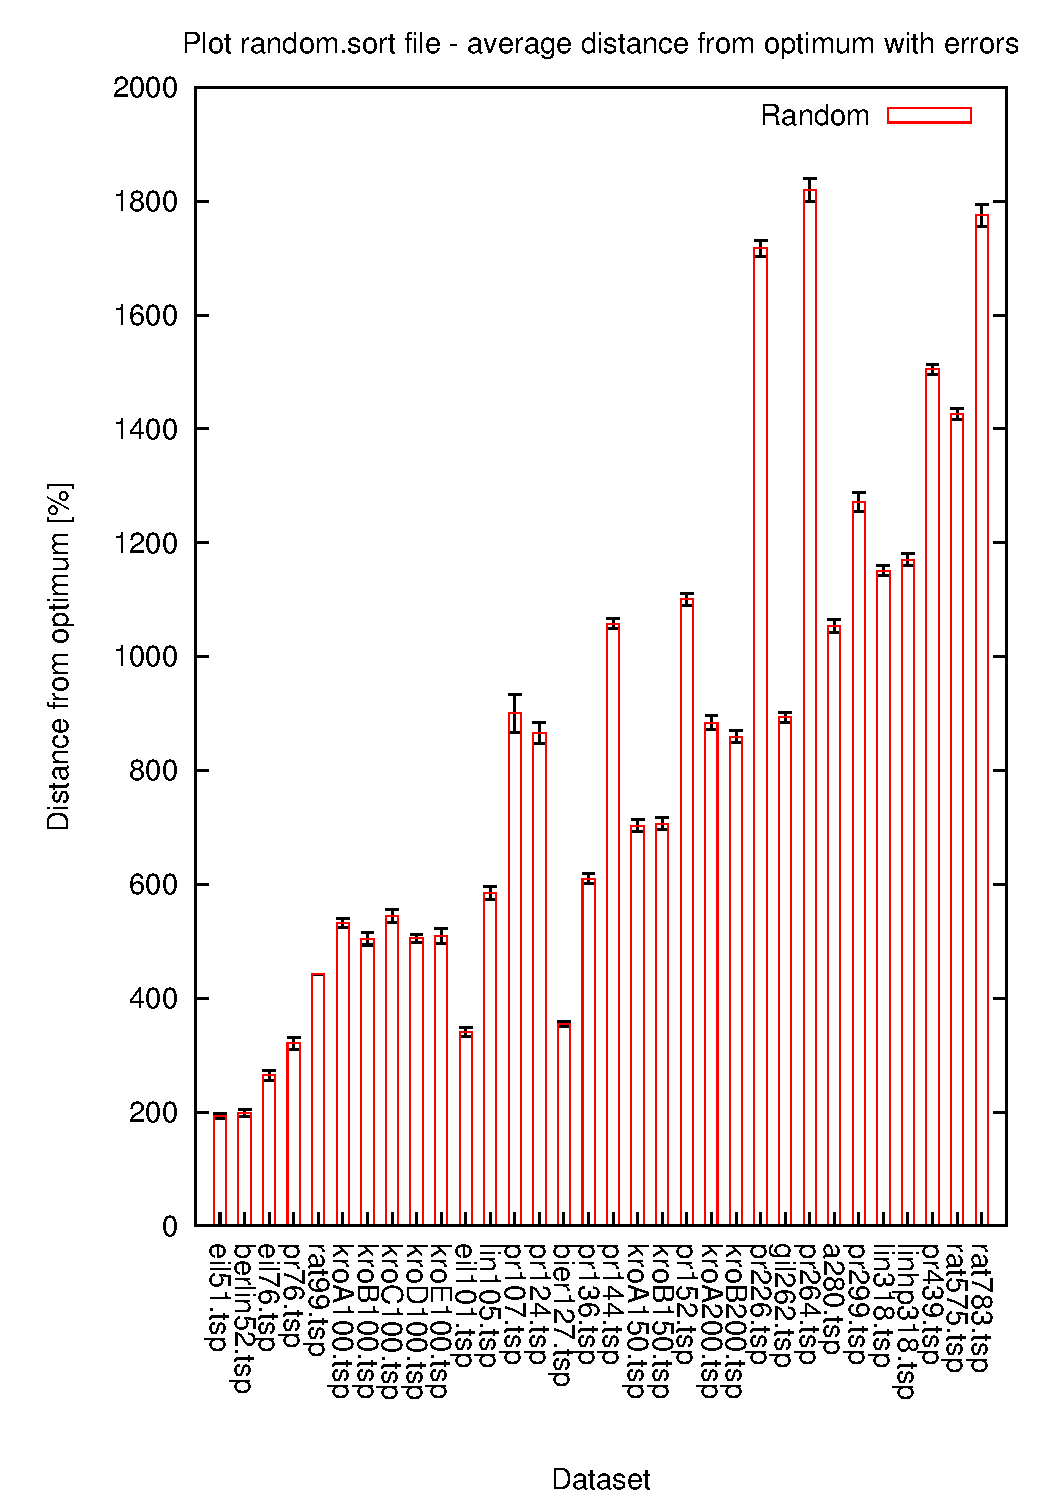
\includegraphics[width=0.9\textwidth]{wykresy/random_av_sort}
\end{center}
\caption{Średnia odległość od optimum dla algorytmu Random.}
\label{random_av_sort}
\end{figure}

\begin{figure}
\begin{center}
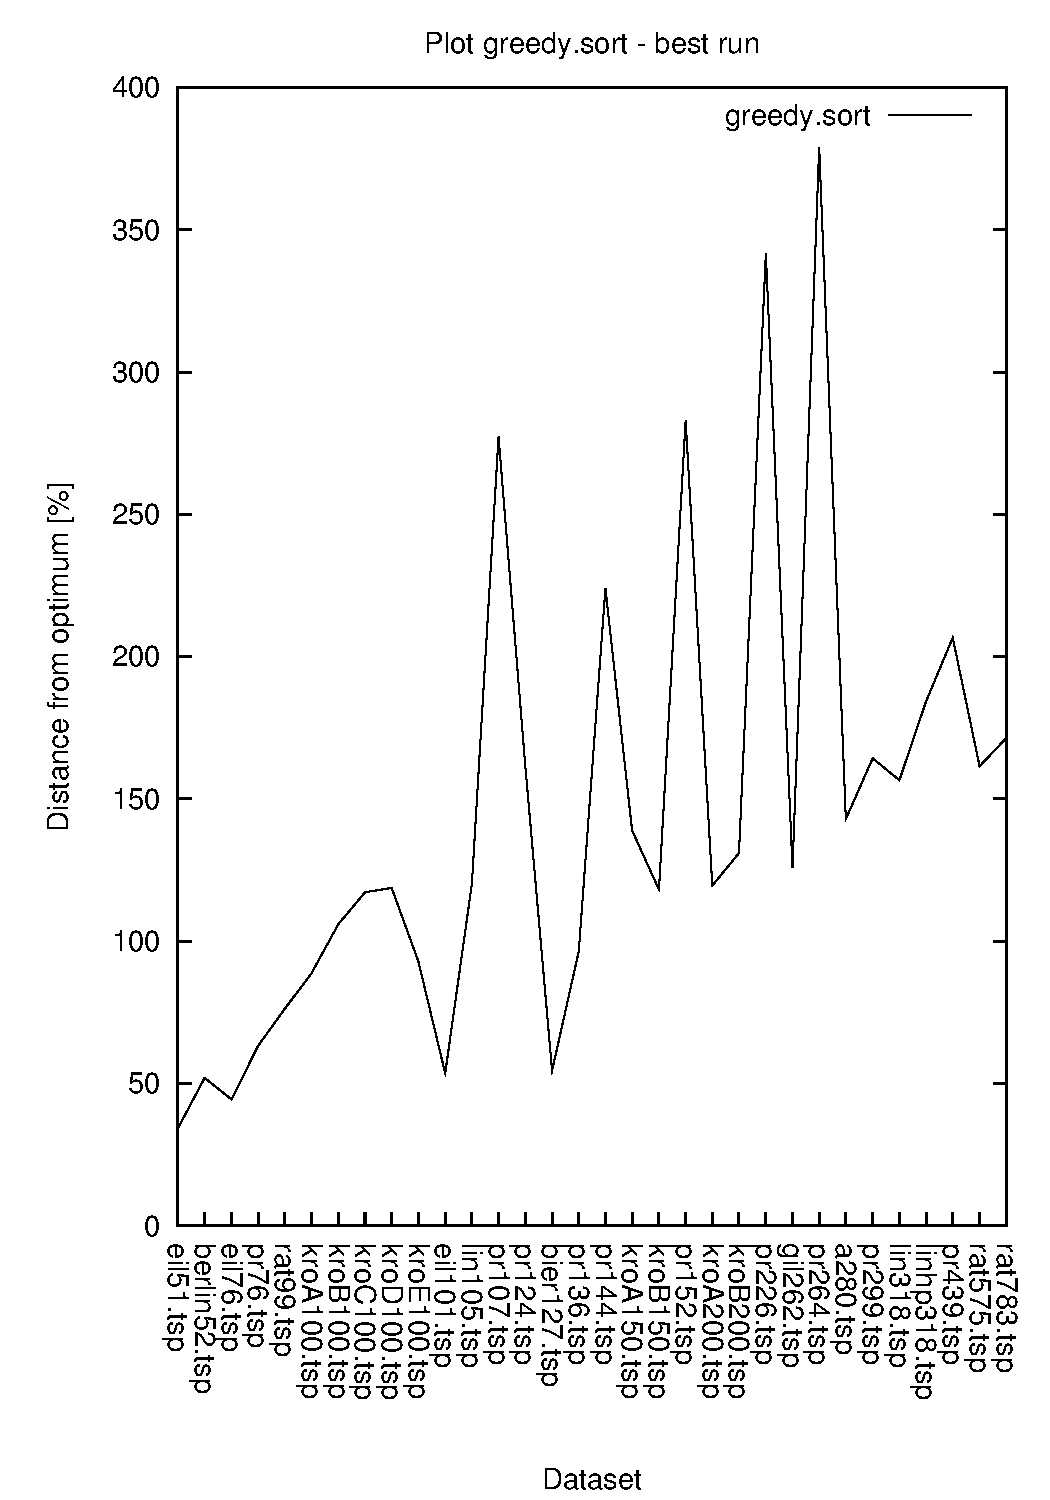
\includegraphics[width=0.9\textwidth]{wykresy/greedy_sort_worst}
\end{center}
\caption{Najgorsza odległość od optimum dla algorytmu Greedy.}
\label{greedy_sort_worst}
\end{figure}


\begin{figure}
\begin{center}
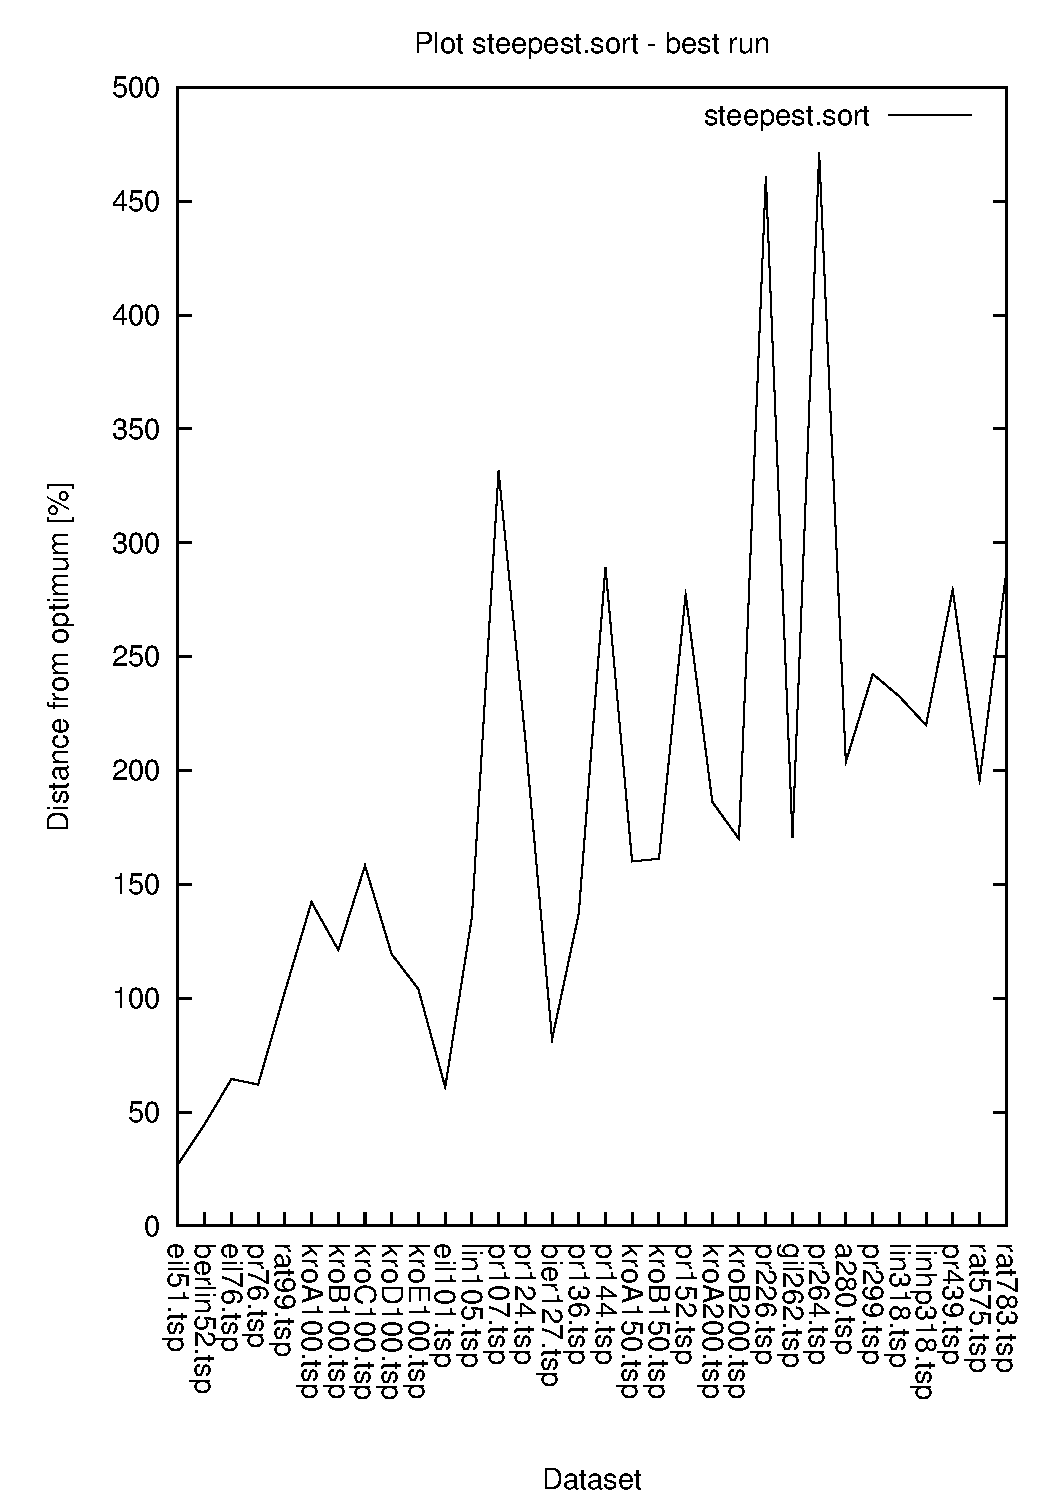
\includegraphics[width=0.9\textwidth]{wykresy/steepest_sort_worst}
\end{center}
\caption{Najgorsza odległość od optimum dla algorytmu Steepest.}
\label{steepest_sort_worst}
\end{figure}

\begin{figure}
\begin{center}
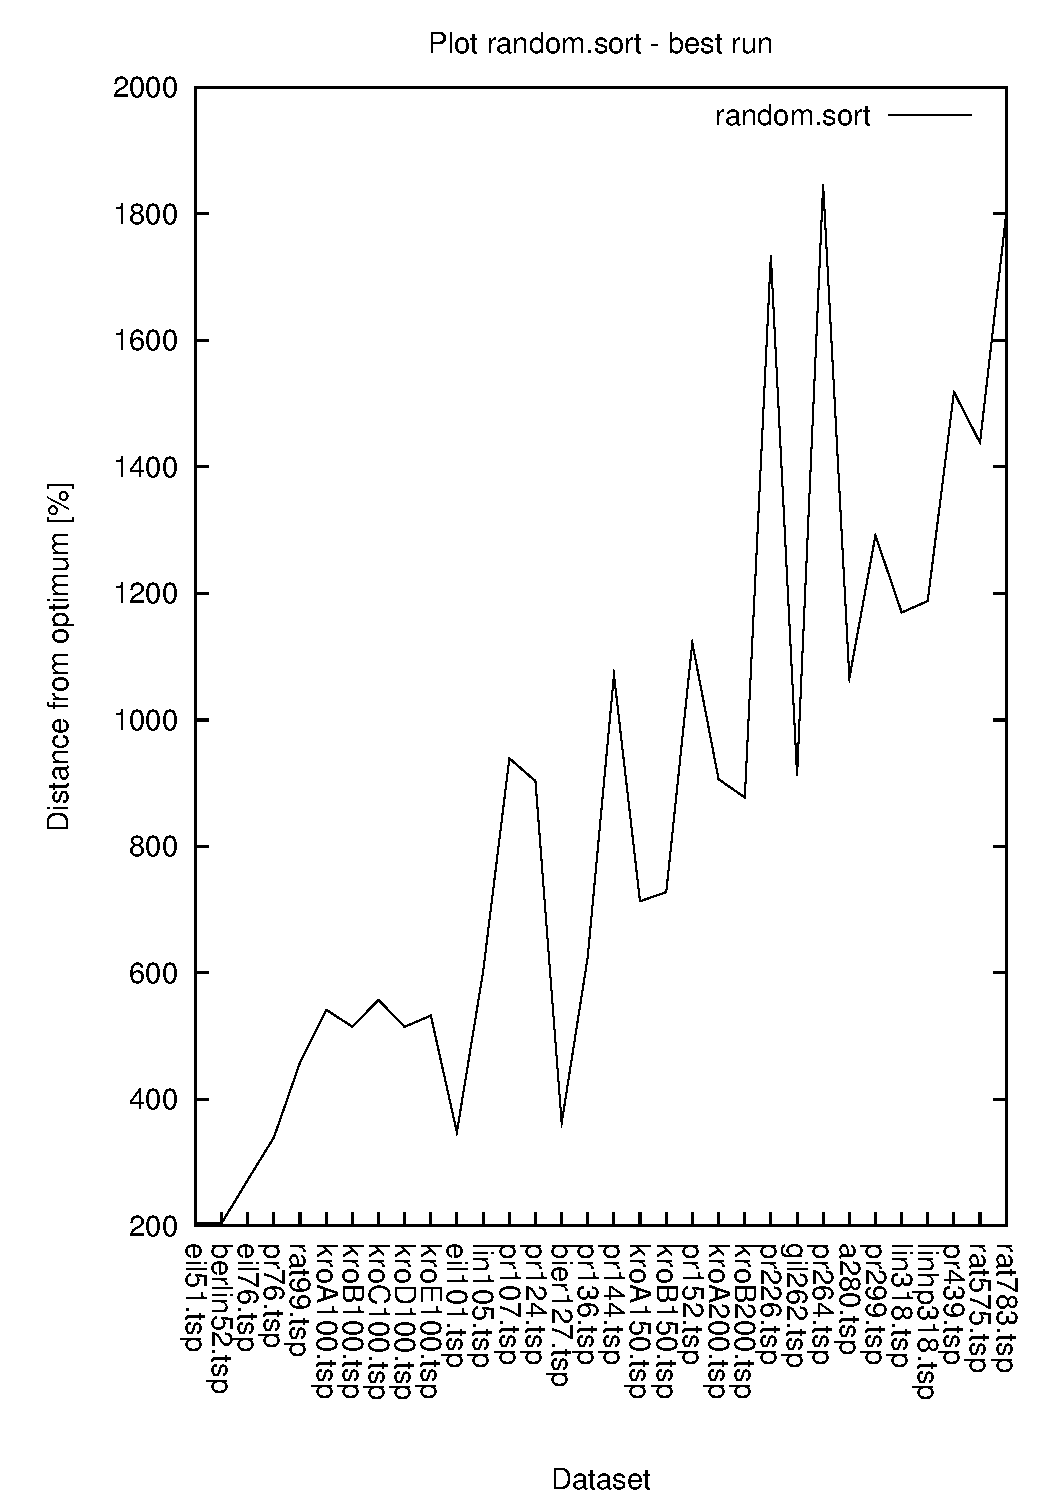
\includegraphics[width=0.9\textwidth]{wykresy/random_sort_worst}
\end{center}
\caption{Najgorsza odległość od optimum dla algorytmu Random.}
\label{random_sort_worst}
\end{figure}



\begin{figure}
\begin{center}
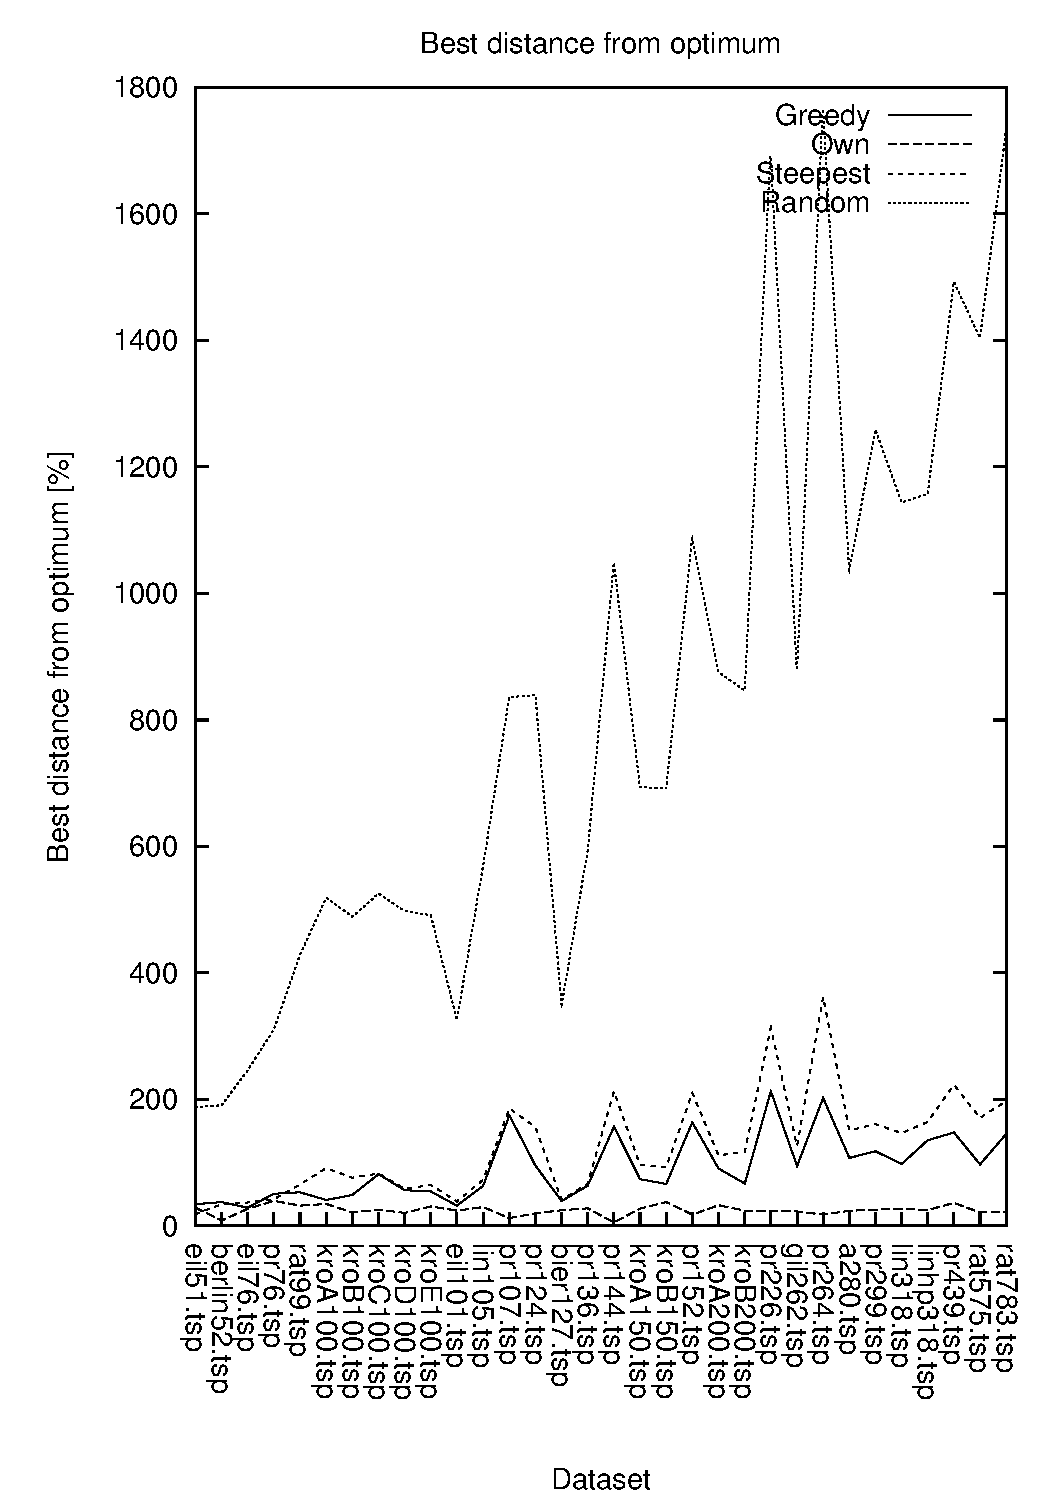
\includegraphics[width=0.9\textwidth]{wykresy/best_com}
\end{center}
\caption{Porównanie algorytmów względem najlepszych uzyskanych wyników.}
\label{best_com}
\end{figure}


\begin{figure}
\begin{center}
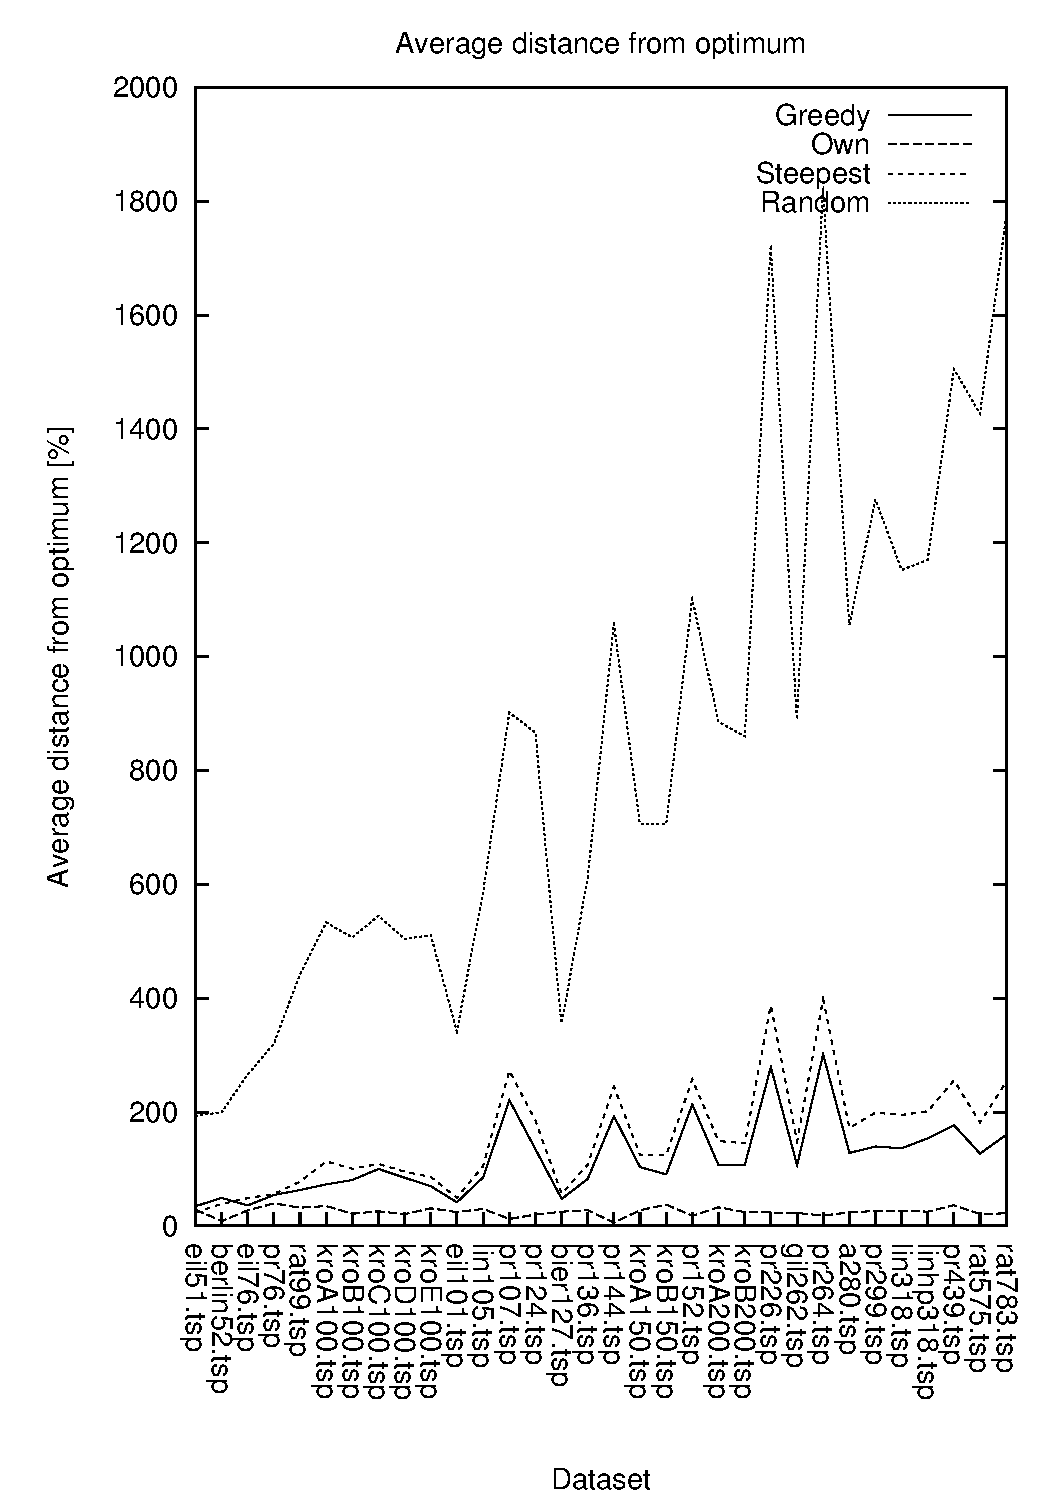
\includegraphics[width=0.9\textwidth]{wykresy/av_comp}
\end{center}
\caption{Porównanie algorytmów względem średnich uzyskanych wyników.}
\label{av_comp}
\end{figure}

\subsection{Jakość/czas}

Zależność jakoś czas postanowiono zmierzyć wg następującego wzoru:

$$ czas\_dzialania * procentowa\_odleglosc\_od\_optimum $$

Uzystane wyniki przedstawiono na rysunkach \ref{greedy_ef}, \ref{steepest_ef} i
\ref{random_ef}.

\begin{figure}
\begin{center}
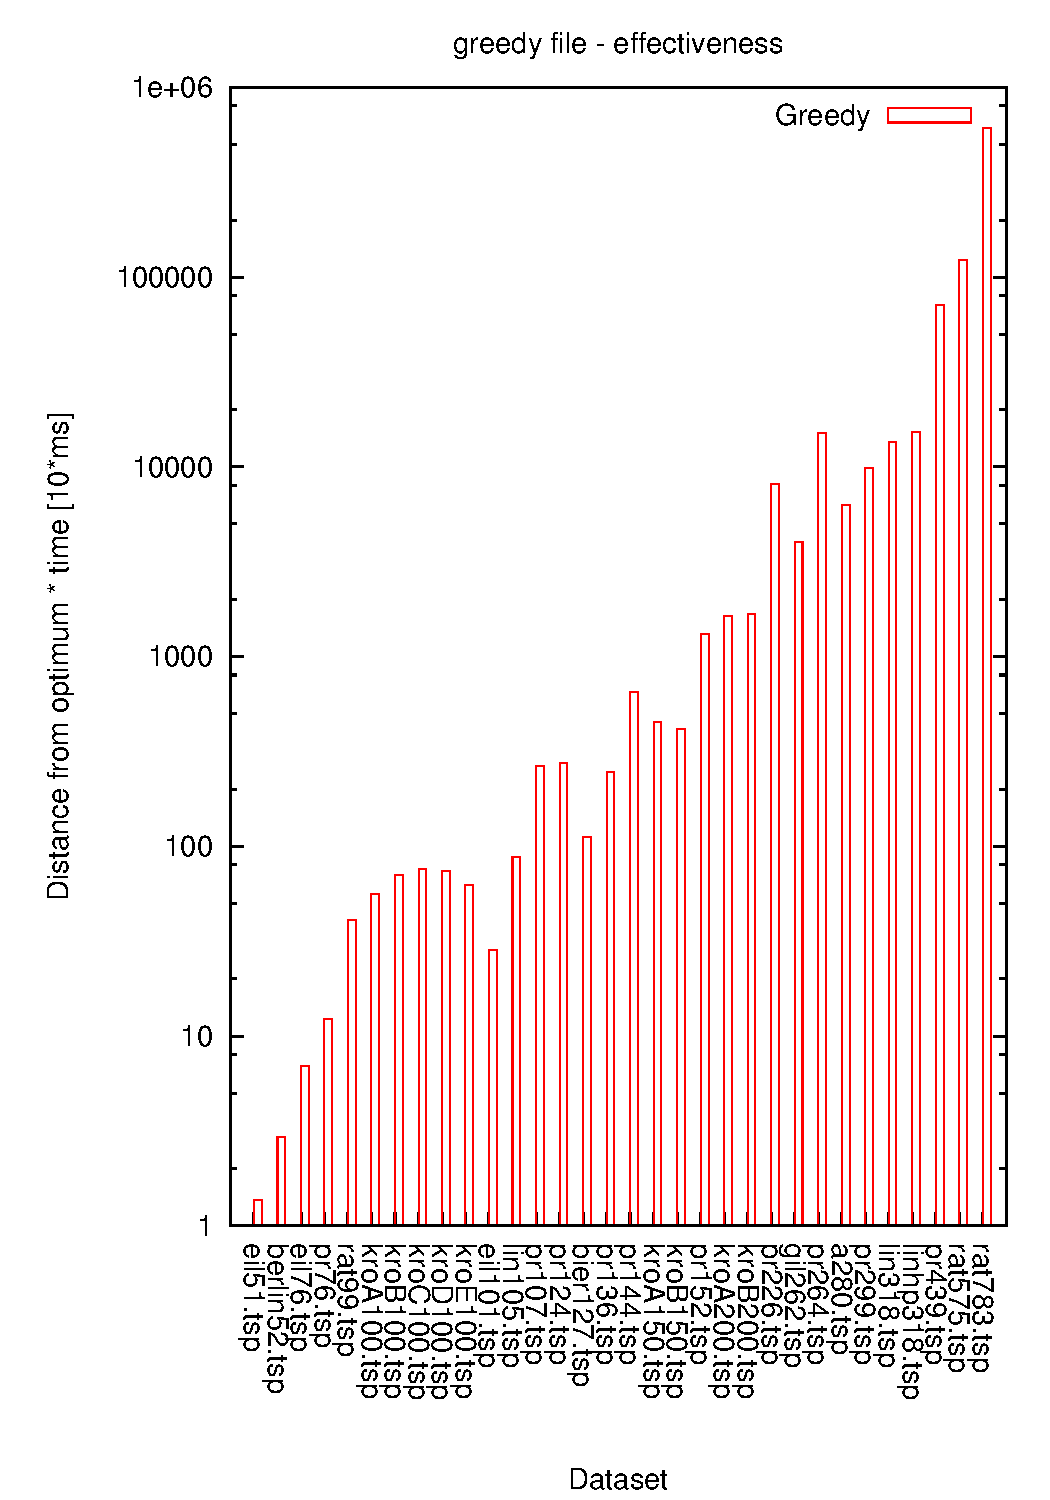
\includegraphics[width=0.9\textwidth]{wykresy/greedy_ef}
\end{center}
\caption{Średnia efektywność algorytmu Greedy.}
\label{greedy_ef}
\end{figure}


\begin{figure}
\begin{center}
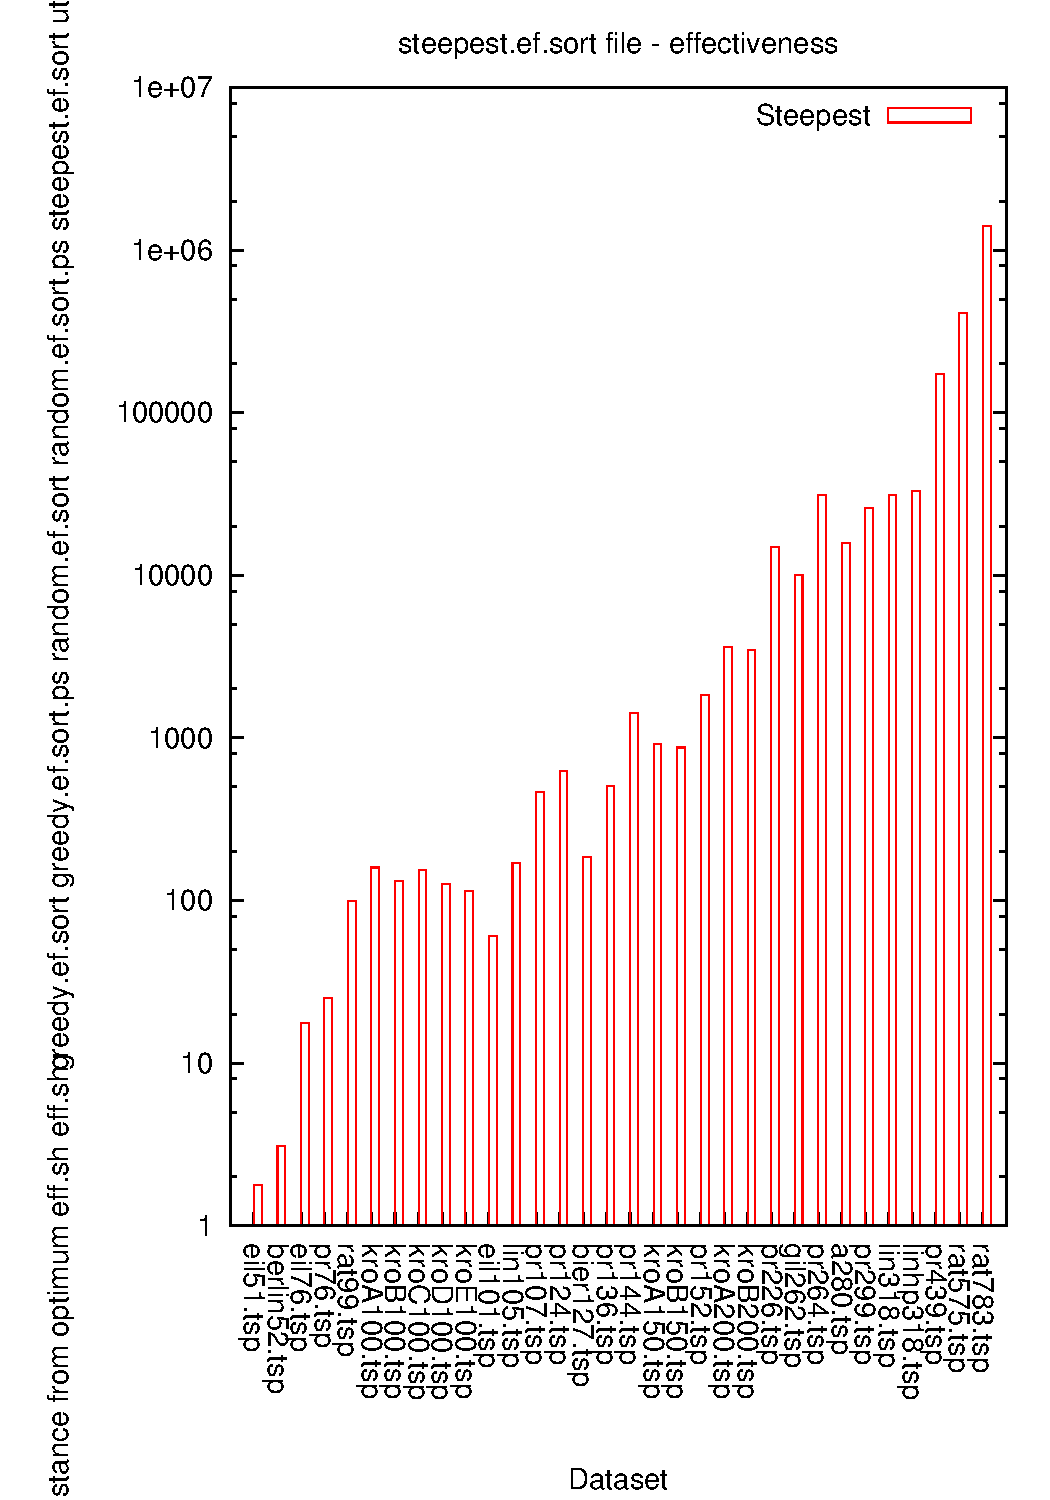
\includegraphics[width=0.9\textwidth]{wykresy/steepest_ef}
\end{center}
\caption{Średnia efektywność algorytmu Steepest.}
\label{steepest_ef}
\end{figure}


\begin{figure}
\begin{center}
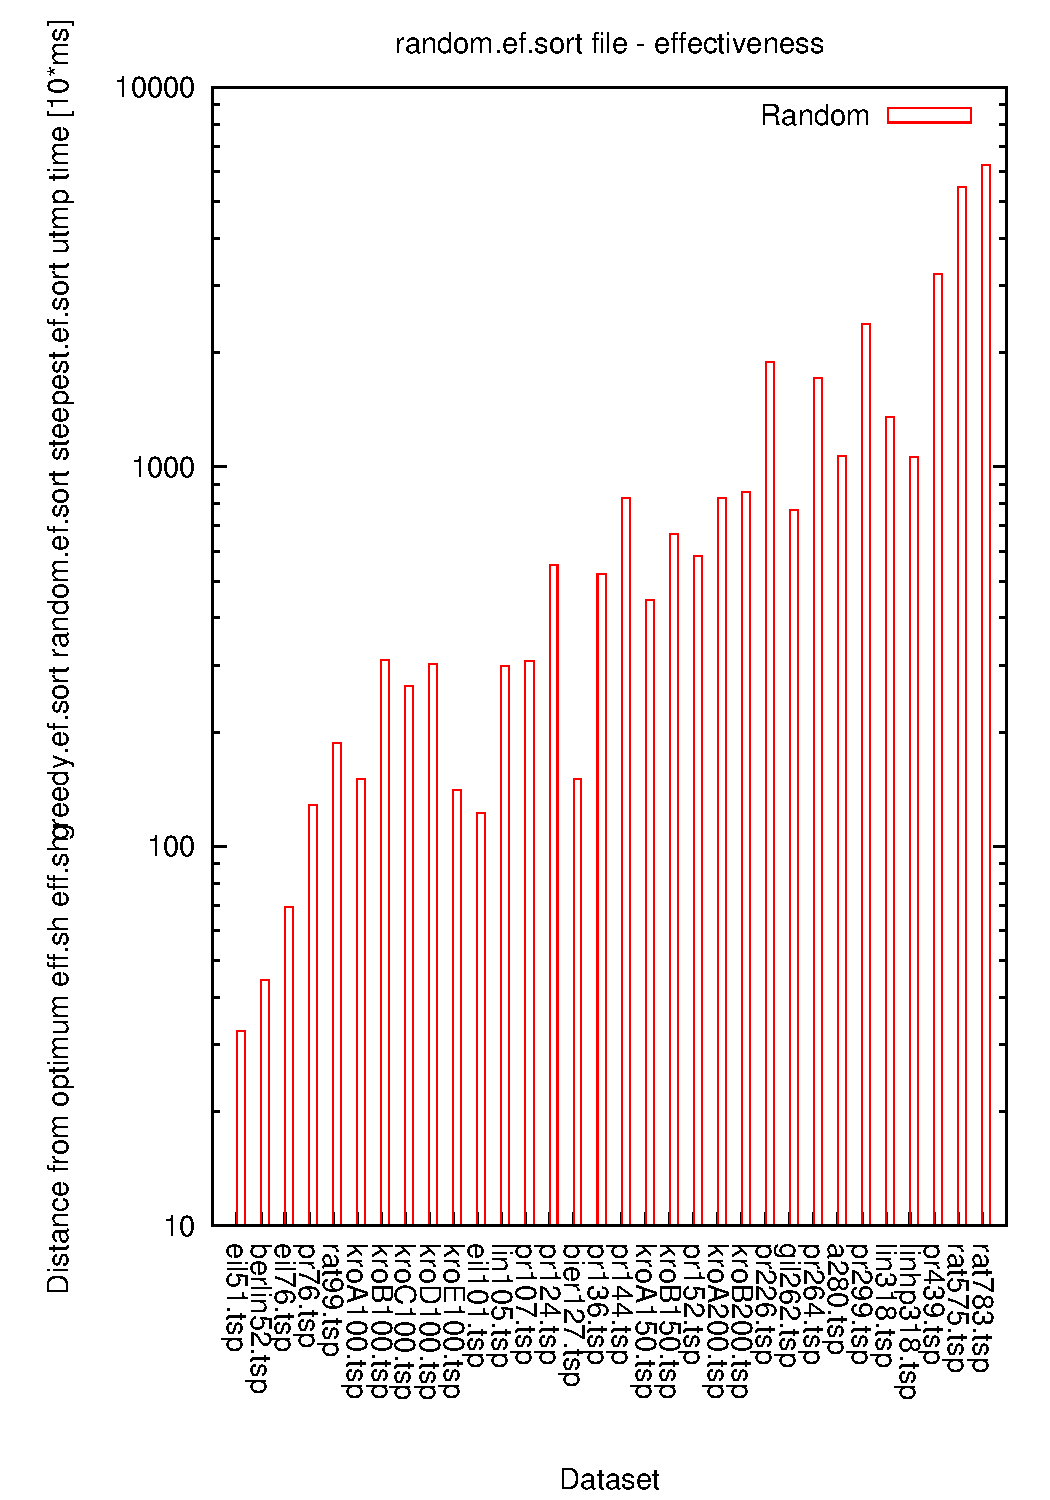
\includegraphics[width=0.9\textwidth]{wykresy/random_ef}
\end{center}
\caption{Średnia efektywność algorytmu Random.}
\label{random_ef}
\end{figure}

\subsection{Czas działania}

Wyniki badań przedstawione zostały na rysunkach \ref{greedy_time} i \ref{steepest_time}.

\begin{figure}
\begin{center}
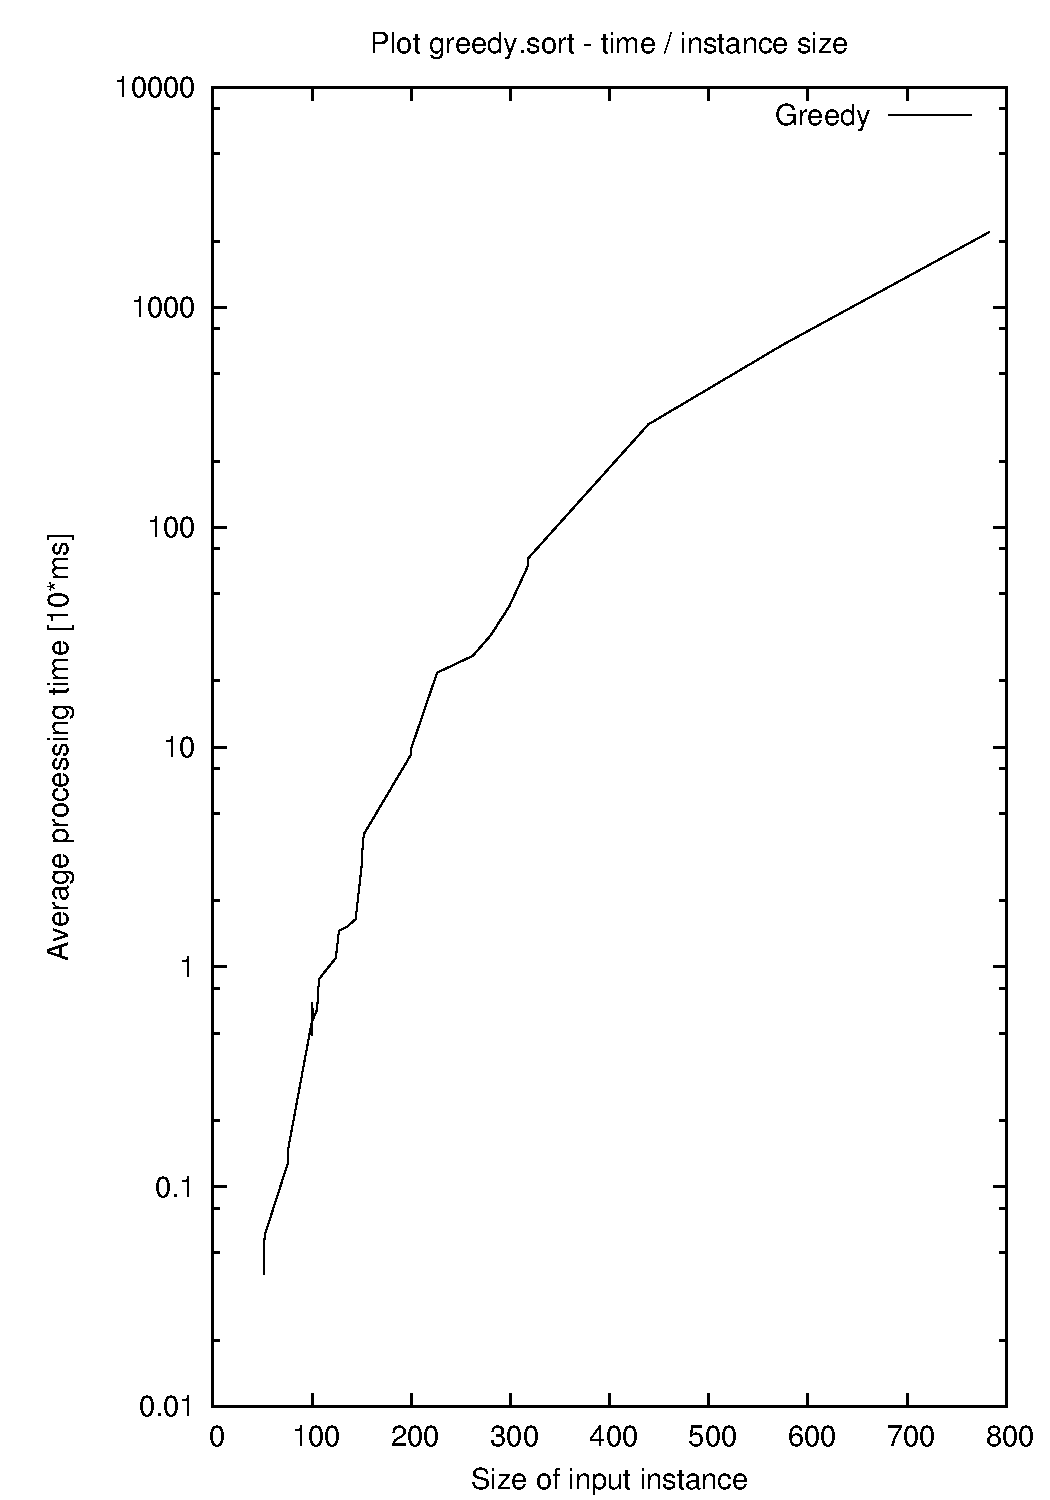
\includegraphics[width=0.9\textwidth]{wykresy/greedy_time}
\end{center}
\caption{Średni czas działania algorytmu Greedy w odniesieniu do rozmiaru instancji.}
\label{greedy_time}
\end{figure}


\begin{figure}
\begin{center}
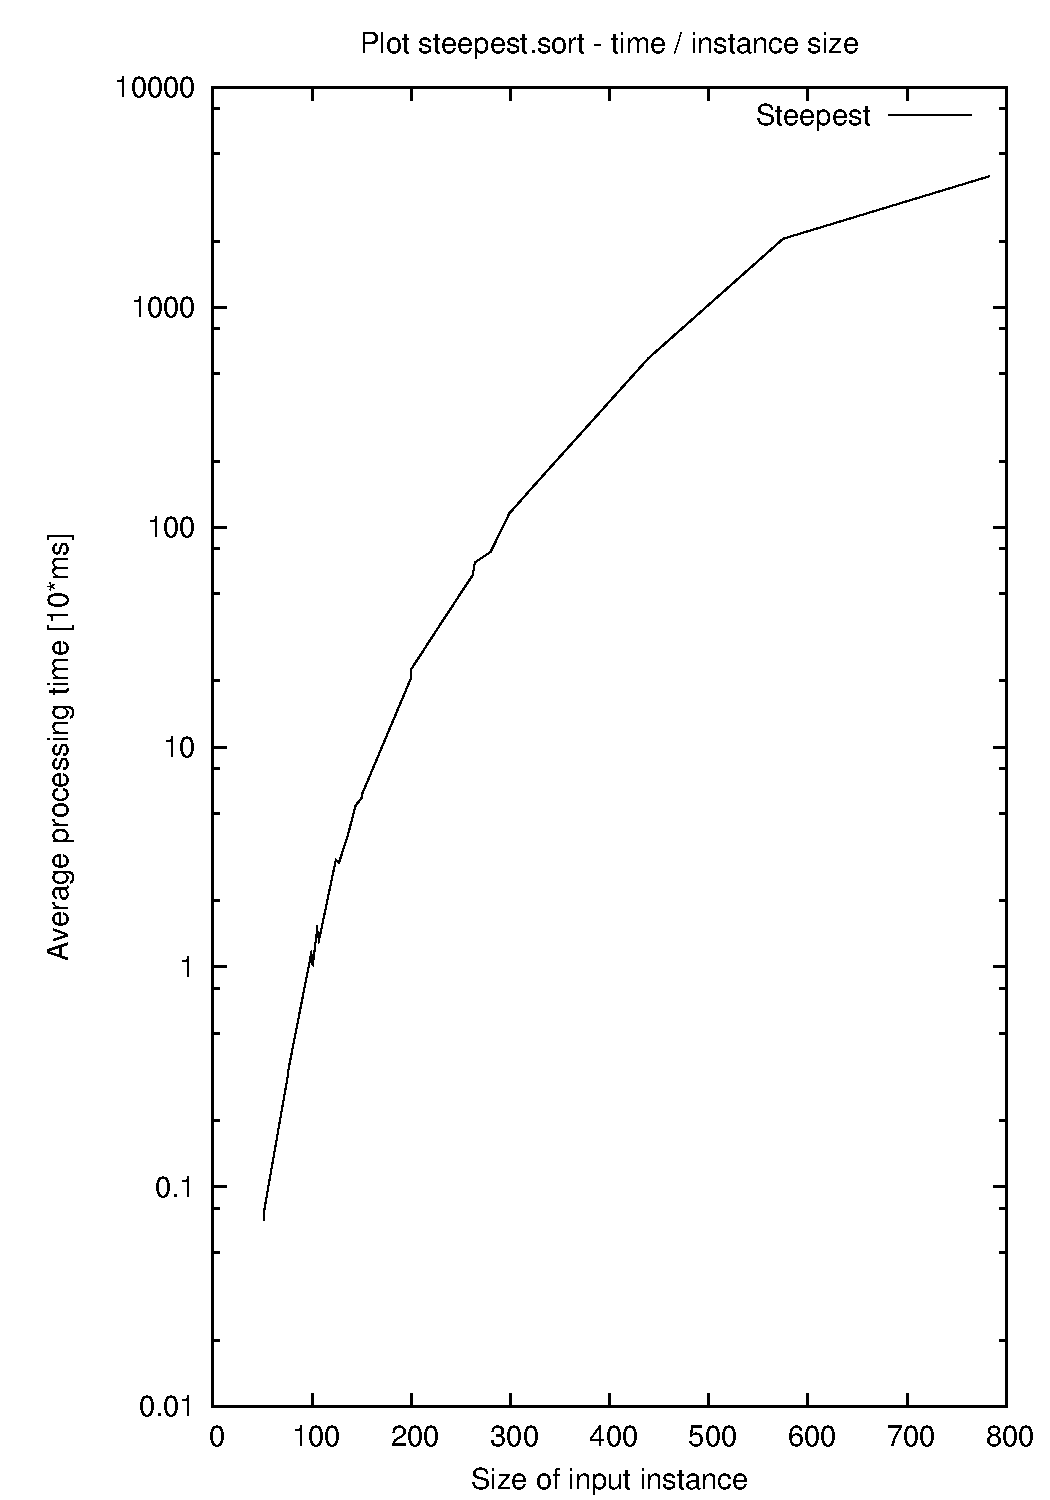
\includegraphics[width=0.9\textwidth]{wykresy/steepest_time}
\end{center}
\caption{Średni czas działania algorytmu Steepest w odniesieniu do rozmiaru instancji.}
\label{steepest_time}
\end{figure}

\subsection{Średnia ilość kroków i przejrzanych algorytmów}

Badania przeprowadzone tylko dla algorytmów Greedy i Steepest. Wyniki uzyskane przedstawione 
zostały na rysunkach \ref{greedy_kroki}, \ref{greedy_sasiedzi}, \ref{steepest_kroki}, \ref{steepest_sasiedzi},
\ref{steps_comp} i \ref{ng_comp}.

\begin{figure}
\begin{center}
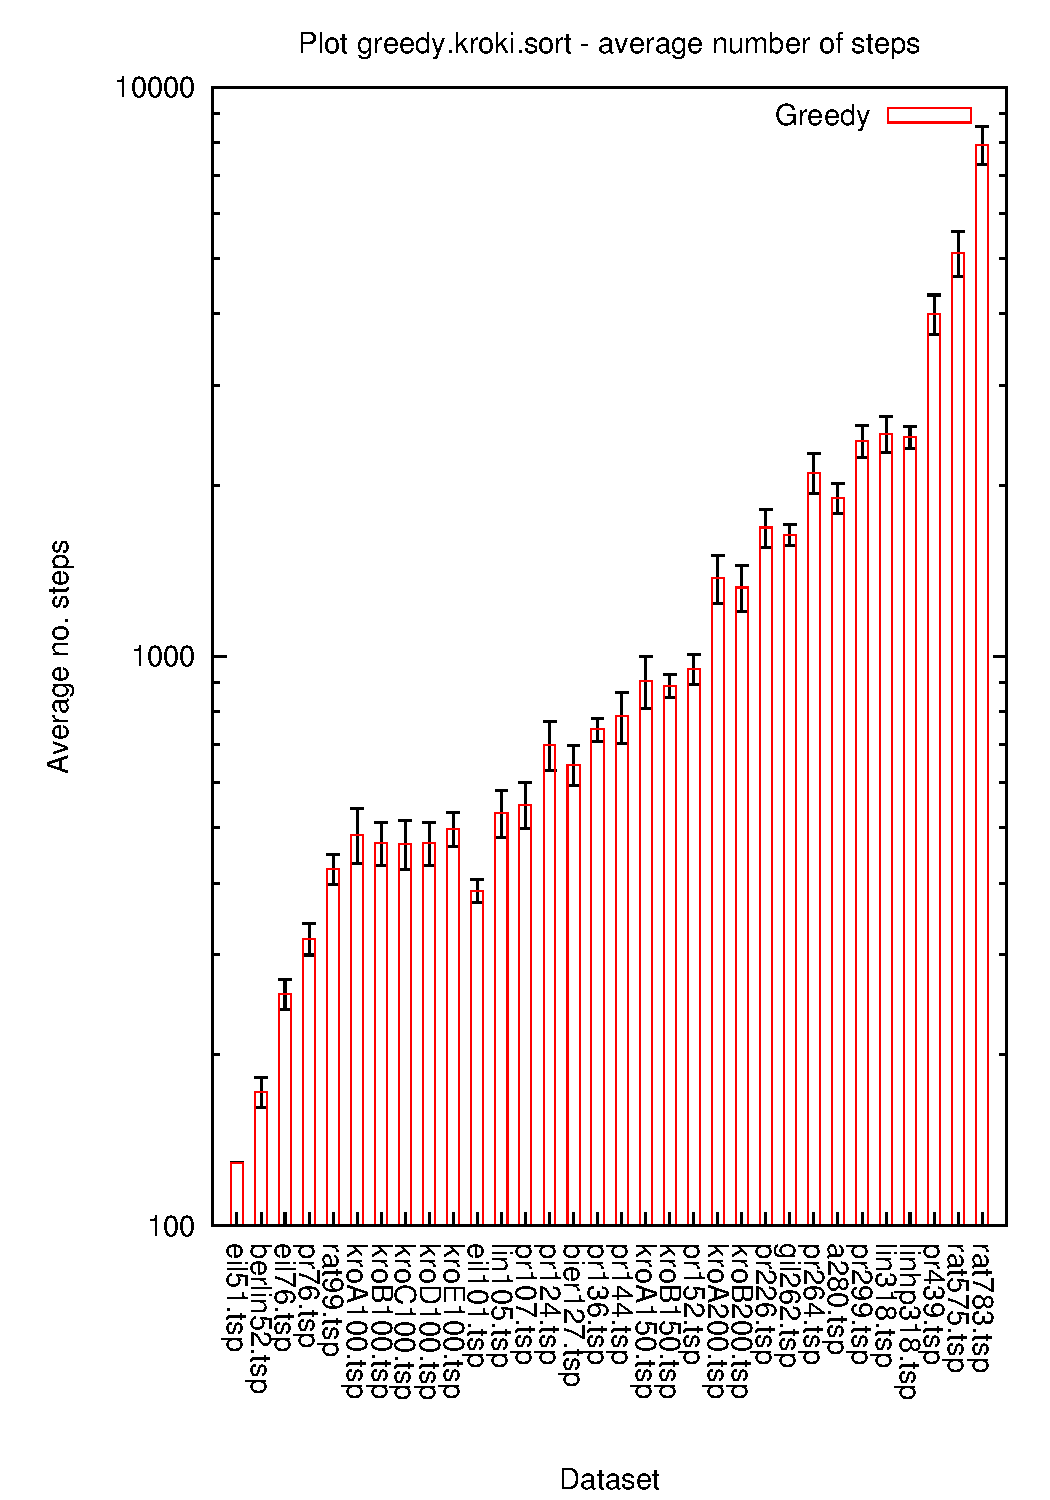
\includegraphics[width=0.9\textwidth]{wykresy/greedy_kroki}
\end{center}
\caption{Średnia ilość kroków wykonanych przez algorytm Greedy wraz z odchyleniem standardowym.}
\label{greedy_kroki}
\end{figure}


\begin{figure}
\begin{center}
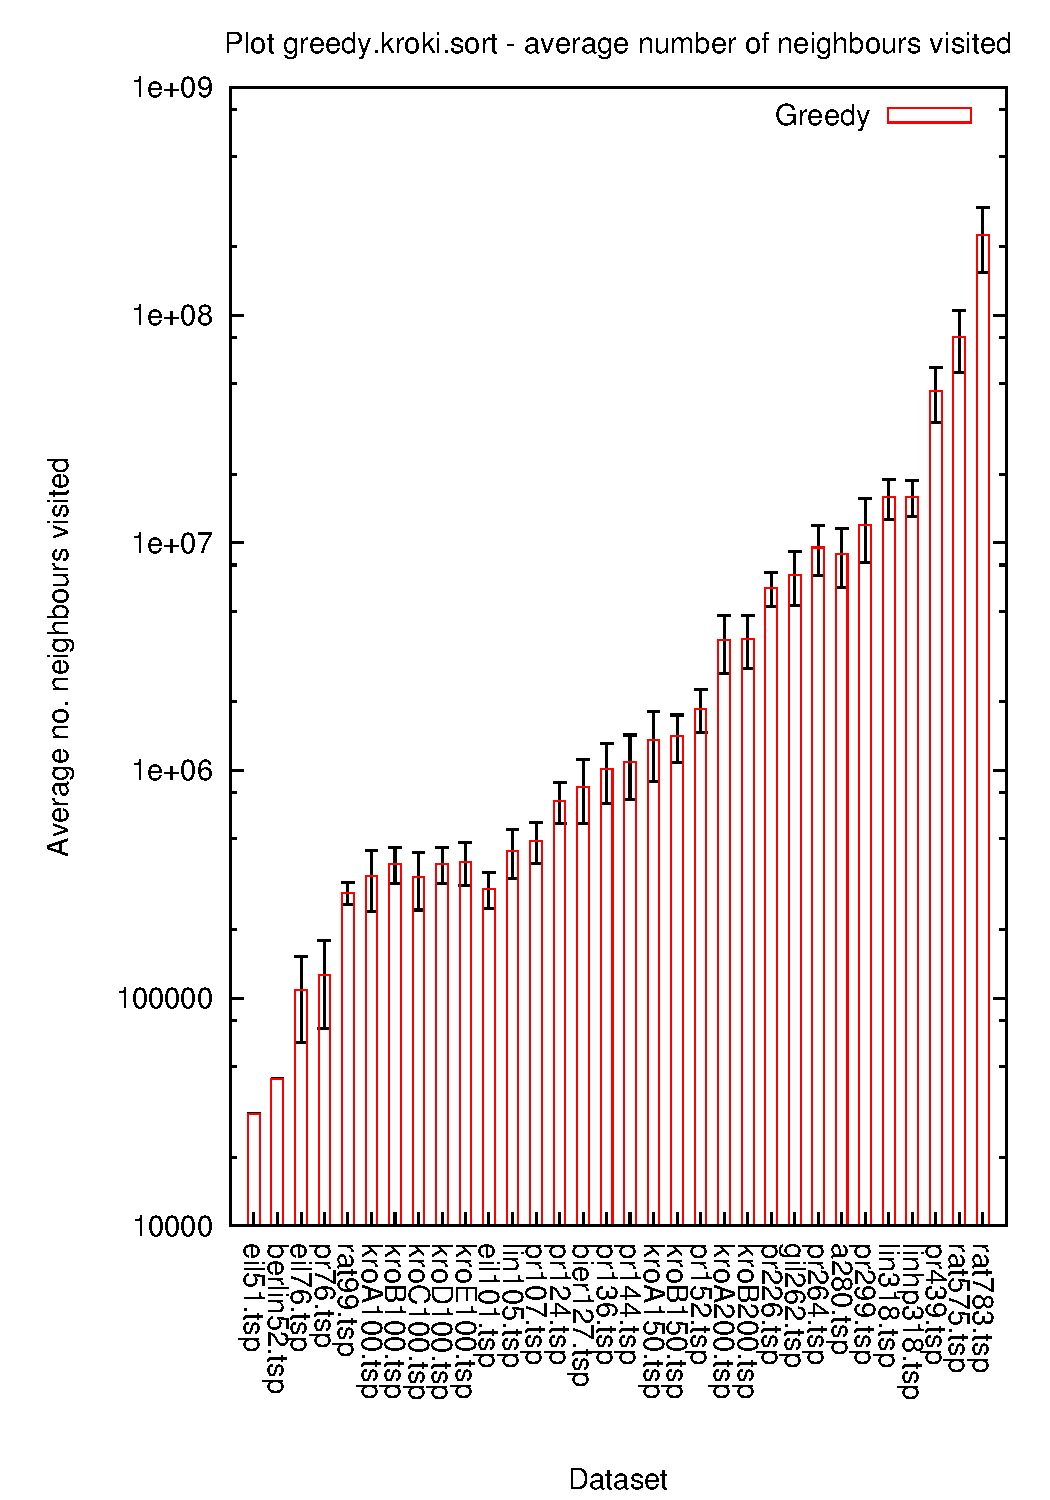
\includegraphics[width=0.9\textwidth]{wykresy/greedy_sasiedzi}
\end{center}
\caption{Średnia ilość rozwiązań przejrzanych przez algorytm Greedy wraz z odchyleniem standardowym.}
\label{greedy_sasiedzi}
\end{figure}

\begin{figure}
\begin{center}
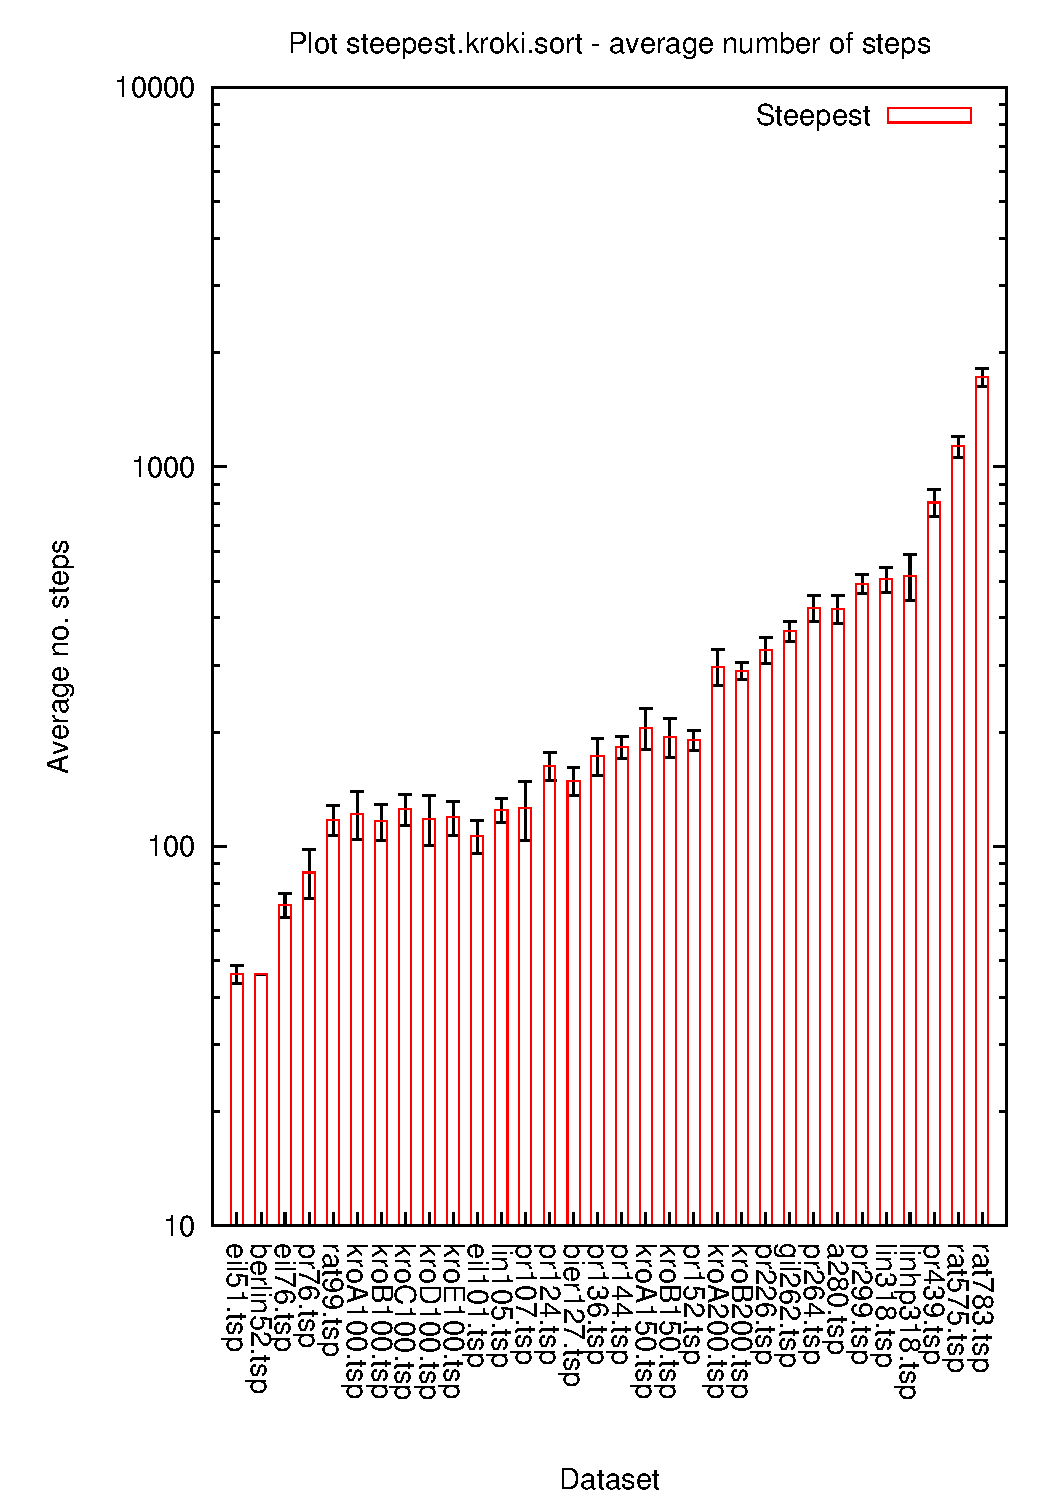
\includegraphics[width=0.9\textwidth]{wykresy/steepest_kroki}
\end{center}
\caption{Średnia ilość kroków wykonanych przez algorytm Steepest wraz z odchyleniem standardowym.}
\label{steepest_kroki}
\end{figure}


\begin{figure}
\begin{center}
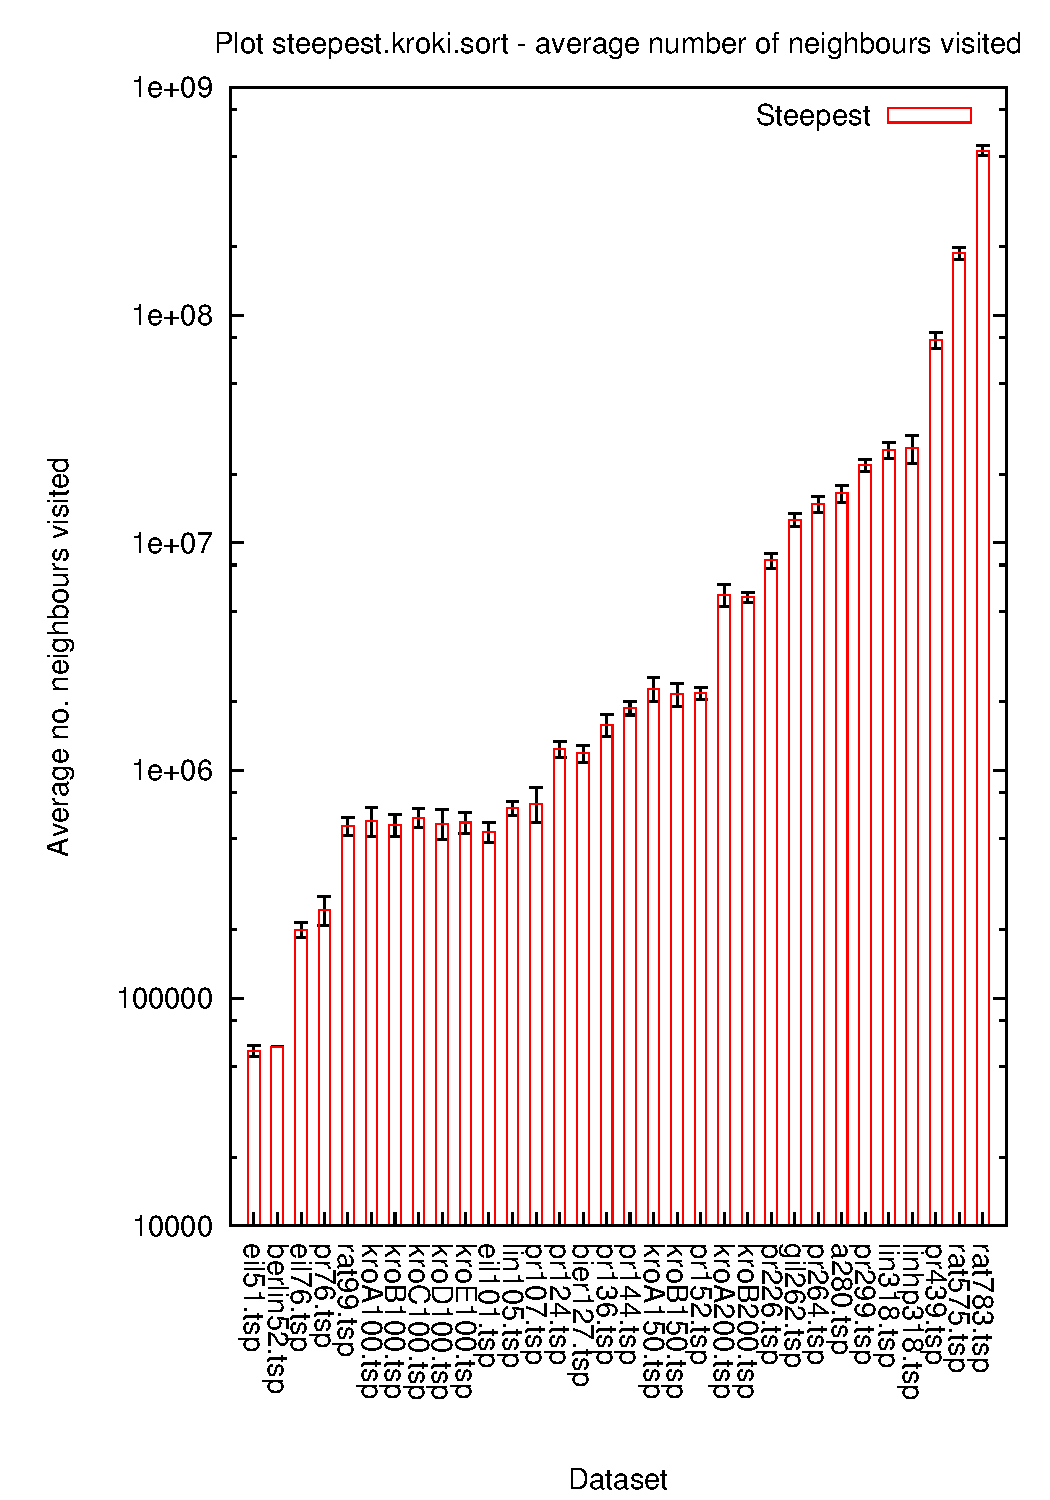
\includegraphics[width=0.9\textwidth]{wykresy/steepest_sasiedzi}
\end{center}
\caption{Średnia ilość rozwiązań przejrzanych przez algorytm Steepest wraz z odchyleniem standardowym.}
\label{steepest_sasiedzi}
\end{figure}


\begin{figure}
\begin{center}
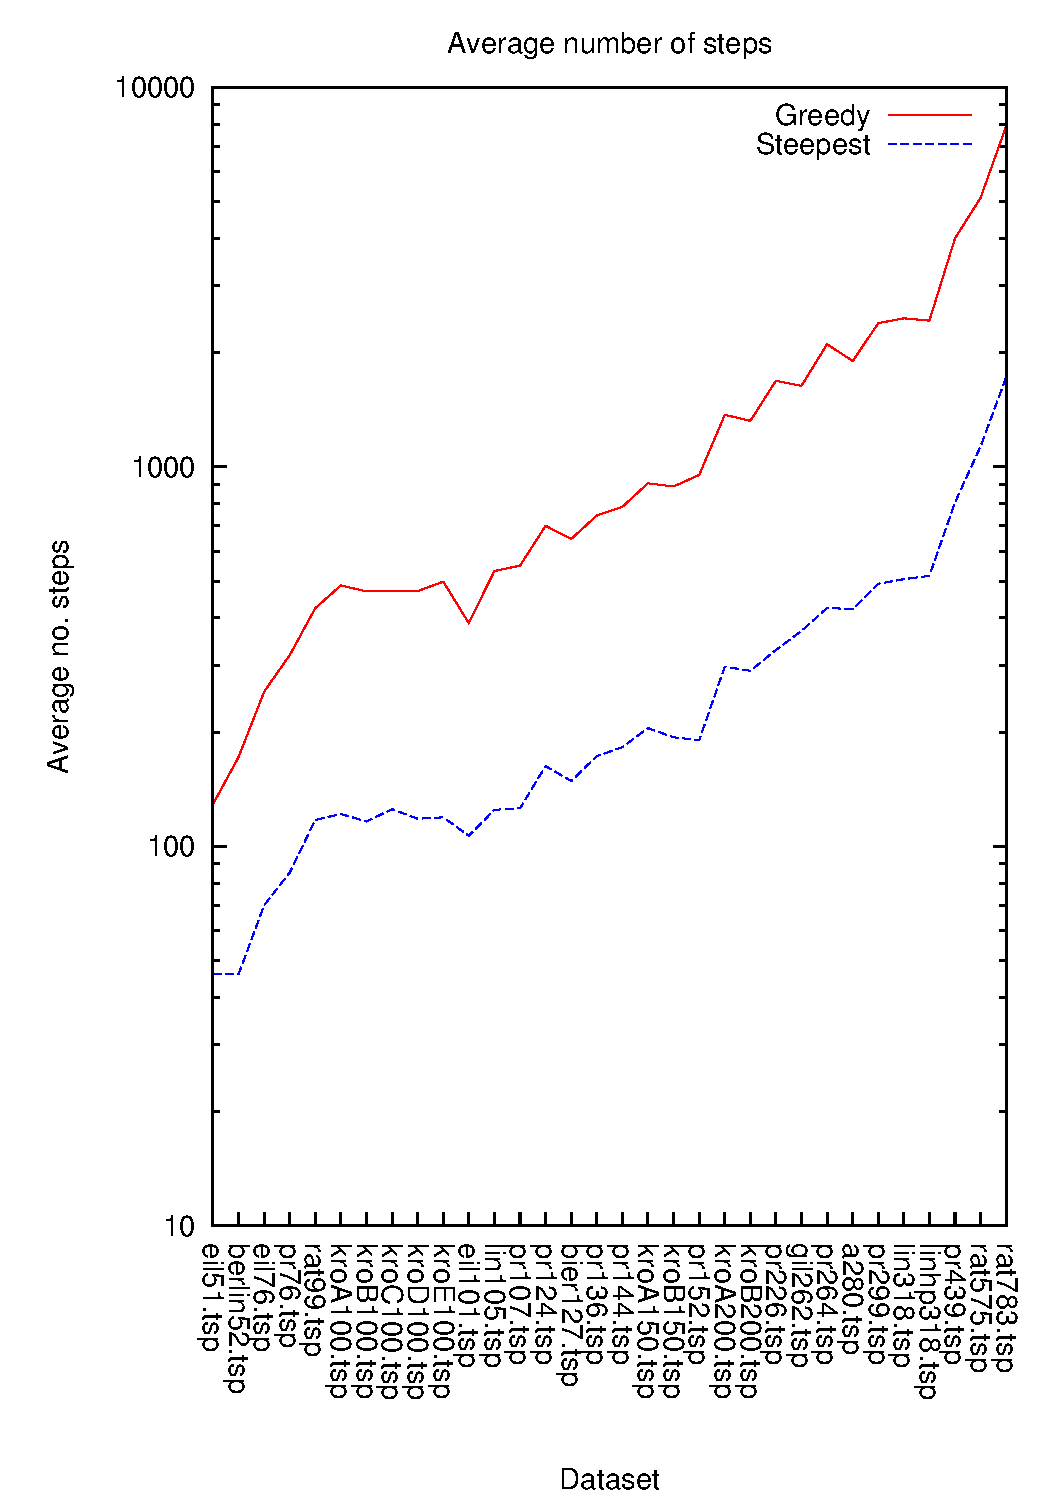
\includegraphics[width=0.9\textwidth]{wykresy/steps_comp}
\end{center}
\caption{Porównanie ilości iteracji rozwiązań przez algorytmy Greedy i Steepes.}
\label{steps_comp}
\end{figure}


\begin{figure}
\begin{center}
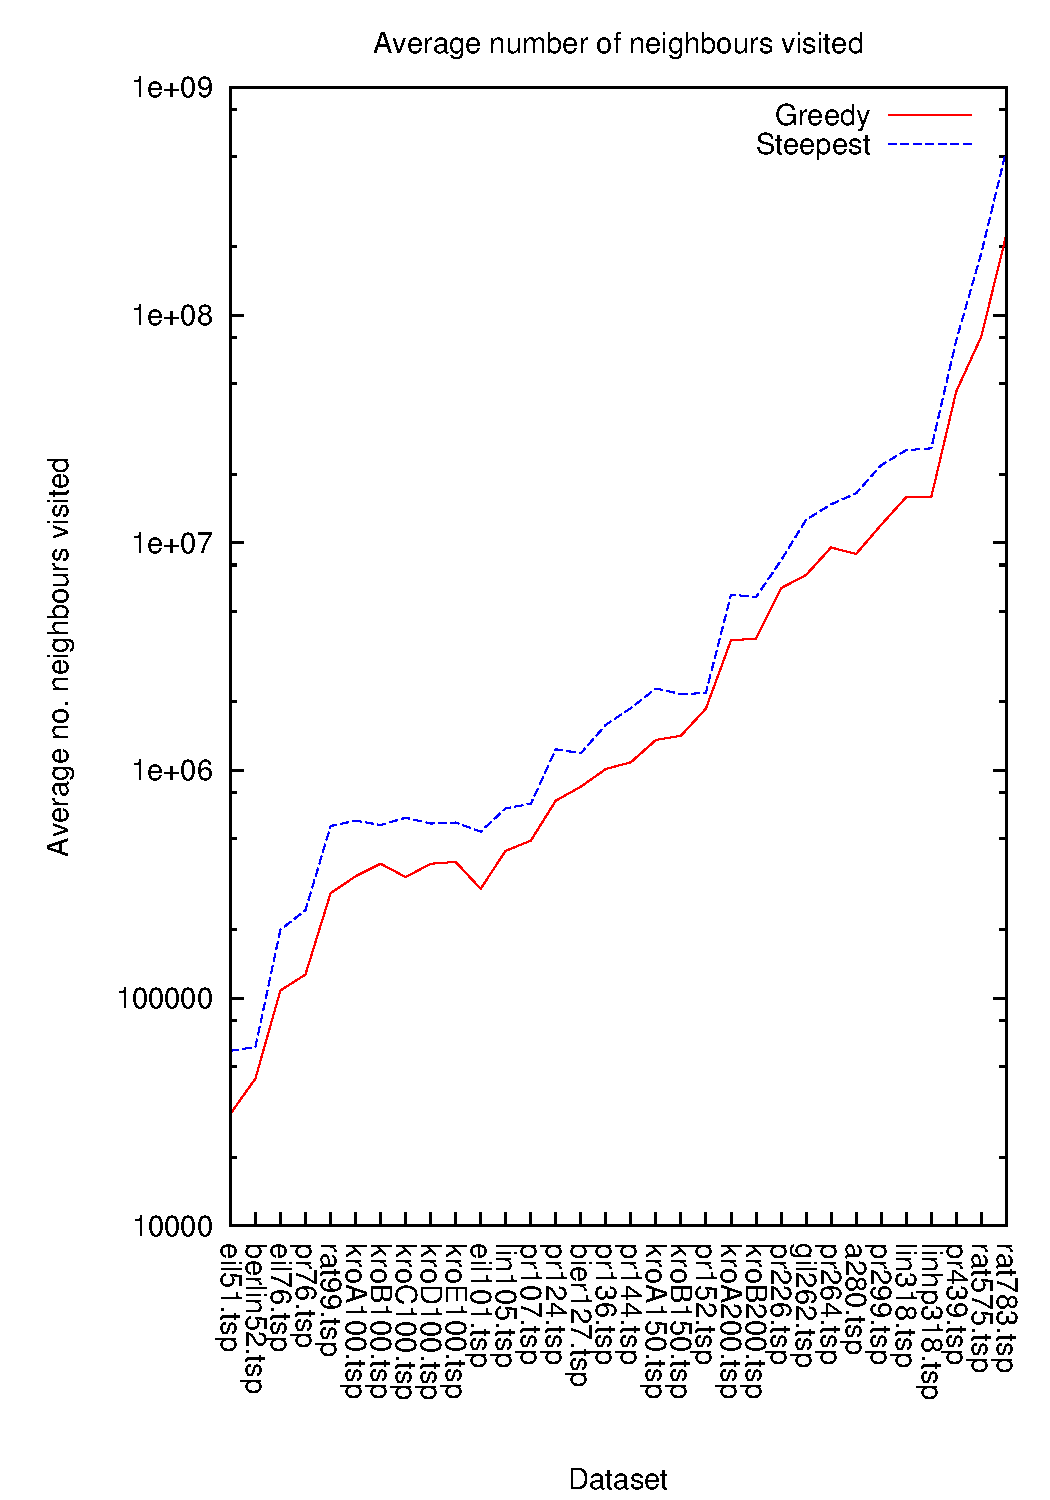
\includegraphics[width=0.9\textwidth]{wykresy/ng_comp}
\end{center}
\caption{Porównanie ilości przejrzanych rozwiązań przez algorytmy Greedy i Steepes.}
\label{ng_comp}
\end{figure}

